\lstset{language=Python}
\usetikzlibrary{svg.path}
\excludecomment{solution}
\tikzset{velox/.style={color=black,draw,fill=red,thick,%
    shape=diamond,aspect=.4,
    inner sep=1.3pt,transform shape}}
\tikzset{veloy/.style={color=black,draw,fill=red,thick,%
    shape=diamond,aspect=2.5,
    inner sep=1.3pt,transform shape}}
\tikzset{veloxy/.style={color=black,draw,fill=red,thick,%
    shape=star,star points=4,star point ratio=2.2,
    inner sep=1.3pt,transform shape}}
\tikzset{pressure/.style={color=black,draw,fill=cyan,thick,%
    shape=circle,inner sep=2pt,transform shape}}
\tikzset{velo/.style={transform shape,double=red,arrows={-Stealth[open,fill=red]}}}

%% Macros for drawing degrees of freedom for different shapes/elements.
%% Arguments are always:
%%   #1: Starting point
%%   #2: End point
%%   #3: polynomial degree
%%   #4: node settings

\tikzset{pics/edgenormal/.style args={#1/#2/#3/#4}{%
    code={%
      \draw #1 -- #2
      node foreach \x [evaluate=\x as \xval] in {1,...,#3} [#4,sloped,pos=\xval/(#3+1)] {};
      }
}}


%% Macros for drawing degrees of freedom for different shapes/elements.
%% Arguments are always:
%%   #1: polynomial degree
%%   #2: node settings

\tikzset{pics/tripile/.style args={#1/#2}{%
    code={%
      \coordinate (top) at (0,#1);
      \foreach \i in{0,...,#1}
      \foreach \j in{0,...,\i}
      {
        \tikzmath{
          \y = .3*(2/3*#1-\i)*cos(30);
          \x = .3*(\i/2-\j);
        }
        \node[#2] at (\x,\y) {};
      }
    }
}}

\tikzset{pics/tensor/.style args={#1/#2/#3}{%
    code={%
      \coordinate (top) at (0,#1);
      \foreach \i in{0,...,#1}
      \foreach \j in{0,...,#2}
      {
        \tikzmath{
          \y = 2*(\i+1)/(#1+2);
          \x = 2*(\j+1)/(#2+2);
        }
        \node[#3] at (\x,\y) {};
      }
    }
}}

\tikzset{pics/pfem/.style args={#1/#2}{%
    code={%
      \tikzmath{ \ytop=2*cos(30); }
      \coordinate (top) at (0,\ytop);

      \foreach \i in{0,...,#1}
      \foreach \j in{0,...,\i}
      {
        \tikzmath{
          \y = \ytop-\ytop*\i/#1;
          \x = 2*(\i/2-\j)/#1+1;
        }
        \node[#2] at (\x,\y) {};
      }
    }
}}

\tikzset{pics/qfem/.style args={#1/#2}{%
    code={%
      \foreach \i in{0,...,#1}
      \foreach \j in{0,...,#1}
      {
        \tikzmath{
          \y = 2-2*\i/#1;
          \x = 2-2*\j/#1;
        }
        \node[#2] at (\x,\y) {};
      }
    }
}}

%%% Local Variables:
%%% mode: latex
%%% TeX-master: "all"
%%% End:


\def\constref#1{C_{\text{\ref{#1}}}}
\title{Einführung in die Numerik}
\author{Guido Kanschat}
\date{\today}

\newcommand{\rd}{\operatorname{rd}}
\newcommand{\eps}{\texttt{eps}}
\begin{document}
\maketitle
\tableofcontents
\chapter{Orthogonale Polynome}
\section{Polynomräume}

% \begin{Satz}{nullstellen}
%   Ein reelles Polynom vom Grad $n$ hat höchstens $n$ Nullstellen oder es ist das Nullpolynom.
% \end{Satz}

% \begin{proof}
%   Für $n=1$ handelt es sich um ein lineares Polynom und die Aussage
%   des Satzes ist unmittelbar klar. Sei nun $p$ ein Polynom strikt vom
%   Grad $n>1$ mit Nullstelle $x_0$. Dann gibt es nach dem euklidischen
%   Algorithmus zur Division mit Rest ein Polynom $q$ vom Grad $n-1$ und
%   eine Konstante $c$, so dass
%   \begin{gather}
%     p(x) = (x-x_0)q(x)+c.
%   \end{gather}
%   Daraus folgt $p(x_0) = c$, so dass folgt $c=0$. Wir können dieses
%   Verfahren für alle weiteren Nullstellen $x_1,\dots,x_m$ wiederholen
%   und erhalten
%   \begin{gather}
%     p(x) =  r(x) \prod_{k=0}^m (x-x_i),
%   \end{gather}
%   wobei $r(x)$ ein Polynom vom Grad $n-m$ sein muss, da $p$ vom Grad
%   $n$ ist. Insbesondere muss gelten $m\le n$.
% \end{proof}

% \begin{Korollar}{polynome-identisch}
%   Zwei reelle Polynome vom Grad $n$ sind identisch, wenn sie in
%   mindestens $n+1$ Punkten übereinstimmen. 
% \end{Korollar}


\begin{Lemma}{monome-linear-unabhaengig}
  Die Menge der Monome $\{x^0, x^1,\dots,x^n\}$ ist linear unabhängig.
\end{Lemma}

\begin{proof}
  Sei $p$ ein Polynom vom Grad $n$, also
  \begin{gather}
     p(x) = a_nx^n+a_{n-1}x^{n-1}+\dots+a_1x+a_0
   \end{gather}
   $p$ ist also gerade eine Linearkombination der Monome.  Zu zeigen
   ist, dass aus der Eigenschaft $p \equiv 0$ folgt, dass alle
   Koeffizienten verschwinden, also
  \begin{gather}
    p(x) \equiv 0
    \quad\Rightarrow\quad a_n = \dots = a_0 = 0.
  \end{gather}
  Zu diesem Zweck berechnen wir die $n$-te Ableitung von $p$ und
  erhalten, da mit $p$ auch alle seine Ableitungen identisch
  verschwinden,
  \begin{gather}
    n! a_n = 0.
  \end{gather}
  Daraus schließen wir $a_n = 0$. Nun gilt für die $(n-1)$-te Ableitung
  \begin{gather}
    n! a_n x + (n-1)! a_{n-1} = (n-1)! a_{n-1} = 0.
  \end{gather}
  Auf diese Weise schließen wir rekursiv bis $a_0$, dass alle Koeffizienten verschwinden. Damit ist das Lemma bewiesen.
\end{proof}

\begin{Satz}{polynomraum}
  Die Polynome vom maximalen Grad $n$ bilden einen Vektorraum der
  Dimension $n+1$.  Wir bezeichnen ihn mit $\P_n$.
\end{Satz}

\begin{proof}
  Es ist leicht nachzurechnen, dass sowohl die Summe, als auch reelle
  Vielfache von Polynomen wieder Polynome sind. Insbesondere erhöhen
  beide Operationen den Grad nicht. Damit ist $\P_n$ ein
  Vektorraum. Er wird per definitionem von den Monomen vom Grad bis zu
  $n$ erzeugt. Da diese nach
  \slideref{Lemma}{monome-linear-unabhaengig} linear unabhängig sind,
  bilden sie eine Basis und die Dimension von $\P_n$ ist $n+1$.
\end{proof}

\begin{Quiz}{Polynomräume}
  Gegeben beliebige Werte $x_j\in\R$ mit $j=1,\dots,n$. Die Menge der
  Polynome $p_i$ definiert durch
  \begin{align*}
    p_0(x) &= 1\\
    p_i(x) &= \prod_{j=1}^i (x-x_j),\qquad i=1,\dots,n
  \end{align*}
  \begin{enumerate}[A]
  \item ist linear unabhängig
  \item ist linear abhängig
  \item ist ein Erzeugendensystem für $\P_n$
  \item ist eine Basis von $\P_n$
  \end{enumerate}
\end{Quiz}
\section{Skalarprodukt und Orthogonalität}
\begin{Definition}{skalarprodukt}
  Sei $V$ ein reeller Vektorraum. Eine Abbildung
  $a\colon V \times V \to \R$ heißt \define{Bilinearform}, wenn für
  $u,v,w\in V$ und $\lambda,\mu\in \R$ gilt
  \begin{align}
    a(\lambda u + \mu v,w) &= \lambda a(u,w) + \mu a(v,w)\\
    a(w,\lambda u + \mu v) &= \lambda (w,u) + \mu a(w,v).
  \end{align}
  Eine Bilinearform heißt \define{symmetrisch}, wenn für $u,v\in V$ gilt
  \begin{gather}
    a(u,v) = a(v,u).
  \end{gather}
  Sie heißt \define{positiv semi-definit}, wenn $a(u,u) \ge 0$ für alle
  $u\in V$ und \define{positiv definit}, wenn zusätzlich
  \begin{gather}
    a(u,u) = 0 \quad \Longrightarrow \quad u=0.
  \end{gather}
  Eine symmetrische, positiv definite Bilinearform heißt
  \define{Skalarprodukt}, in der Regel notiert als $\scal(\cdot,\cdot)$.
\end{Definition}

%%%%%%%%%%%%%%%%%%%%%%%%%%%%%%%%%%%%%%%%%%%%%%%%%%%%%%%%%%%%%%%%%%%%%%
\begin{Lemma*}{bcs}{Bunjakowski-Cauchy-Schwarzsche Ungleichung}
  Sei $\scal(\cdot,\cdot)$ ein Skalarprodukt auf $V$.  Für zwei beliebige Elemente $u,v\in V$ gilt
  \begin{gather}
    \abs{\scal(u,v)} \le \sqrt{\scal(u,u)} \, \sqrt{\scal(v,v)}.
  \end{gather}
  Gleichheit gilt genau dann, wenn $u$ und $v$ kollinear sind, also
  $v=\alpha u$ mit einem skalaren Faktor $\alpha$.
\end{Lemma*}

\begin{proof}
  Zunächst zeigen wir nur die Ungleichung: Für $v=0\in V$ ist sie
  offensichtlich.
  
  Seien nun $v,u \in V$ keine Nullvektoren. Für beliebige $\mu, \lambda \in \R$
  gilt wegen der Bilinearität 
  \begin{gather}
   0 \le \scal(\lambda u + \mu v,\lambda u +  \mu v)
    = \lambda^{2} \scal(u,u)+2 \mu \lambda \scal(u,v) +\mu^{2} \scal(v,v)
  \end{gather}
  Setze $\lambda := \scal(v,v) \neq 0$
  \begin{gather}
   0 \le \scal(v,v)^{2} \scal(u,u) + 2\mu \scal(v,v)\scal(u,v) +\mu^{2}\scal(v,v)
  \end{gather}
  Dividiere durch$\scal(v,v)$
  \begin{gather}
   0 \le \scal(v,v) \scal(u,u) + 2\mu \scal(u,v) +\mu^{2}
  \end{gather}
  Setze nun $\mu := -\scal(u,v)$
  \begin{gather}
    0 \le \scal(v,v) \scal(u,u) -2\scal(u,v)^{2}+\scal(u,v)^{2}
  \end{gather}
  Daraus folgt
  \begin{gather}
    \scal(u,v)^{2} \le \scal(u,u) \scal(v,v)
  \end{gather}
  und mit der Monotonie der Quadratfunktion die Ungleichung.

  Nun bleibt die Äquivalenz für die Gleichheit zu zeigen.
  Für $v=0$ ist dies wieder trivial erfüllt. Seien zunächst $u,v$ linear abhängig, also zum Beispiel $u=av$.
  Dann gilt mit der Abkürzung $f(v) = \sqrt{\scal(v,v)}$
  \begin{gather}
    \abs{\scal(u,v)} = \abs{\scal(av,v)}
    = \abs{a} \cdot f(v) \cdot f(v)
    = f(av) \cdot f(v) =f(u) \cdot f(v).
  \end{gather}

  Gelte nun umgekehrt $\scal(u,v) = \sqrt{\scal(u,u)}\sqrt{\scal(v,v)}$.
  Es folgt
  \begin{gather}
     \scal(v,v) \scal(u,u) -2\scal(u,v)^{2}+\scal(u,v)^{2} = 0.
  \end{gather}
  Setze $\mu = \scal(u,v)\neq 0 $ und
  $\lambda = \scal(v,v)\neq 0$. Dann erhält man
  \begin{gather}
    \lambda \scal(u,u) - 2 \mu \scal(u,v) + \mu^2 = 0.
  \end{gather}
  Multipliplikation mit $\scal(v,v)$ ergibt
  \begin{gather}
   \lambda^2 \scal(u,u)+2\mu \scal(u,v)\scal(v,v) +\mu^{2}\scal(v,v) = 0 = \scal(\lambda u-\mu v,\lambda u-\mu v).
  \end{gather}
  
  Wegen der Definitheit folgt nun
  $\lambda u + \mu v = 0$ und da $\mu$ und $\lambda$ ungleich Null sind gilt,
  dass $ u,v$ linear abhängig sind
\end{proof}

%%%%%%%%%%%%%%%%%%%%%%%%%%%%%%%%%%%%%%%%%%%%%%%%%%%%%%%%%%%%%%%%%%%%%%
\begin{Lemma}{hilbertnorm}
  Sei $V$ ein reeller Vektorraum mit Skalarprodukt
  $\scal(\cdot,\cdot)$. Dann ist durch
  \begin{gather}
    \norm{u} = \sqrt{\scal(u,u)}
  \end{gather}
  auf $V$ eine Norm definiert. Ein reeller Vektorraum $V$ mit
  Skalarprodukt und zugehöriger Norm heißt \define{euklidischer
    Vektorraum}.
\end{Lemma}

\begin{proof}
  Das Skalarprodukt ist nicht negativ, daher ist die Abbildung $\norm{\cdot}\colon V \to \R$ wohldefiniert.
  Wir müssen nun die Normeigenschaften nachrechnen. Sei dazu $u \in V$. Es gilt
  \begin{enumerate}
  \item Nichtnegativität und Definitheit folgen sofort aus den entsprechenden Eigenschaften des Skalarprodukts.
  \item Homogenität
  \begin{gather}
    \norm{\lambda u} = \sqrt{\scal(\lambda u,\lambda u)}
    =\sqrt{\lambda^{2}\scal(u,u)}
    = \abs{\lambda}\sqrt{\scal(u,u)}
    =\abs{\lambda}\norm{u}
  \end{gather}
  \item Deiecksungleichung
  \begin{gather}
    \begin{aligned}
      \norm{u+v}^{2}
      &= \scal(u+v,u+v)\\
      &= \scal(u,u)+ 2 \scal(u,v) + \scal(v,v)\\
      \label{eq:orthopoly:1}
      &\le \scal(u,u)+ 2 \norm{u} \, \norm{v} + \scal(v,v)\\
      &=\norm{u}^{2}+ 2 \norm{u} \, \norm{v}+ \norm{v}^{2}\\
      & =(\norm{u}+\norm{v})^{2}\\
    \end{aligned}
  \end{gather}
  Daraus folgt durch Wurzelziehen auf beiden Seiten $\norm{u+v} \le \norm{u}+\norm{v}$.
  Für die Abschätzung in Zeile~\eqref{eq:orthopoly:1} haben wir die
  Bunyakovsky-Cauchy-Schwarz-Ungleichung aus \slideref{Lemma}{bcs} verwendet.
  \end{enumerate}
\end{proof}

\begin{Lemma*}{l2-norm}{$L^2$-Skalarprodukt}
  Auf dem Raum $V=\P_n$ der reellen Polynome vom Grad bis zu $n$ ist durch
  \begin{gather}
    \scal(p,q) = \int_{-1}^1 p(x)q(x)\dx
  \end{gather}
  ein Skalarprodukt definiert. Dieses wird $L^2$ Skalarprodukt genannt.
\end{Lemma*}

\begin{proof}
  Hier gilt es zu prüfen, ob die Abbildung auch die vier Eigenschaften eines
  Skalarprodukts erfüllt.\\
  Seien  $p,q,g \in \P_n$ in diesem Beweis.\\
  Da wir schon von einem Skalarprodukt ausgehen, empfiehlt es sich
  zuerst die Symmetrie zu zeigen.
  \begin{gather}
    \scal(p,q) =  \int_{-1}^1 p(x)q(x)\dx = \int_{-1}^1 q(x)p(x)\dx
    =\scal(q,p)
  \end{gather}
  Wenn wir nun zeigen, dass es eine Bilinearform ist müssen wir nur noch eine
  Identität zeigen, da wir schon wissen, dass die Symmetrieeigenschaft
  erfüllt ist.
  \begin{gather}
    \begin{aligned}
    \scal(\lambda p + \mu q, g)
    &= \int_{-1}^1 (\lambda p(x)+ \mu q(x))g(x)\dx\\
   & = \int_{-1}^1 \lambda p(x)g(x)+ \mu q(x)g(x)\dx \\
   &= \int_{-1}^1 \lambda  p(x)g(x)\dx + \int_{-1}^1 \mu q(x)g(x)\dx \\
   &= \lambda \int_{-1}^1 p(x)g(x)\dx + \mu  \int_{-1}^1 q(x)g(x)\dx \\
   &= \lambda \scal(p,g) + \mu \scal(q,g)
    \end{aligned}
  \end{gather}
  Da wir die Symmetrie vorher gezeigt haben, gilt Linearität auch
  im zweiten Argument.\\
  
  Als letztes zeigen wir, dass die Abbildung positiv definit ist.
  \begin{gather}
    0 = \scal(p,p) = \int_{-1}^1 p(x)p(x)\dx =\int_{-1}^1 p(x)^{2}\dx
  \end{gather}
  Aus den Integraleigenschaften folgt
  \begin {gather}
    0 = p(x)^{2} \quad \forall x
  \end{gather}
  Dies kann nur der Fall sein, wenn $p \equiv 0$ ist.\\
  Somit haben wir nachgerechnet, dass es sich um Skalarprodukt handelt.
  \end{proof}

\begin{Definition}{l2-norm}
  Nach dem \slideref{Lemma}{hilbertnorm} können wir mit diesem Skalarprodukt eine Norm auf $\P_n$
  definierten. Diese Norm wird als die $L^2$ Norm bezeichnet.
  \begin{gather}
    \norm{f}_{L^2} = \sqrt{\scal(f,f)_{L^2}} = \int_{-1}^1 f(x)^2 dx
  \end{gather}
  \end{Definition}

\begin{Definition}{orthogonal}
  Zwei Vektoren $u,v\in V$ heißen \define{orthogonal}, wenn
  \begin{gather}
    \scal(u,v) = 0.
  \end{gather}
  Ein Vektor $u\in V$ ist orthogonal zum Untervektorraum $W\subset V$, wenn
  \begin{gather}
    \scal(u,v) = 0\quad\forall v\in W.
  \end{gather}
\end{Definition}

\begin{Notation}{euklidischer-vr}
  Von nun an bezeichnet $V$ immer einen endlichdimensionalen, reellen,
  euklidischen Vektorraum.
\end{Notation}

\begin{Lemma*}{pythagoras}{Pythagoras}
  Seien zwei Vektoren $u\in V$ und $v\in V$ orthogonal zueinander. Dann gilt
  \begin{gather}
    \norm{u+v}^{2} = \norm{u}^{2} + \norm{v}^{2}
  \end{gather}
\end{Lemma*}

\begin{proof}
  Seien $u,v \in V$. Es gilt $ 0 = \scal(u,v)$
   \begin{gather}
    \norm{u+v}^{2} = \scal(u+v,u+v)
    %=\scal(u+v,u)+\scal(u+v,v)
    %=\scal(u,u)+\scal(v,u)+\scal(u,v)+\scal(v,v)
    =\norm{u}^{2} + \norm{v}^{2} +2\scal(u,v) = \norm{u}^{2} + \norm{v}^{2}
  \end{gather}
\end{proof}

\section{Bestapproximation und orthogonale Projektion}
\begin{Definition}{bestapproximation}
  Sei $A\subset V$ ein affiner Unterraum eines euklidischen
  Vektorraums. Dann ist die Bestapproximation $u_b\in A$ eines Vektors
  $u\in V$ in $A$ definiert durch die Beziehung
  \begin{gather}
    \norm{u-u_b} = \min_{v\in A} \norm{u-v}.
  \end{gather}
\end{Definition}

\begin{Satz}{bestapproximation}
  Sei $w \in V$ und $W \subset V$.
  Sei $A=w+W$ ein nichtleerer, affiner Unterraum von $V$. Dann
  existiert die Bestapproximation nach
  \slideref{Definition}{bestapproximation} und ist eindeutig
  bestimmt. Es gilt die notwendige und hinreichende Bedingung
  \begin{gather}
    \scal(u-u_b,v) = 0 \quad \forall v\in W.
  \end{gather}
  Das heißt $ u_b$ ist Bestapproximation genau dann wenn $u-u_b$
  orthogonal zu $W$ bzgl. des Skalarprodukts $\scal(\cdot,\cdot)$ ist.
\end{Satz}

\begin{proof}
  Der Beweis gliedert sich in drei Teile. Zuert wird die Äquivalenz
  gezeigt danach zeigen wir die Eindeutigkeit und zum Schluss
  erst die Existenz.\\ \\
 $\glqq \Rightarrow \glqq$
  Sei $ u_b \in A$ die Bestapproximation des Vektors $ u \in V$\\
  Wir defnieren nun eine Funktion:
  \begin{gather}
    F_v(x):= \norm{u-u_b-xv}^{2}, x \in \R,  v\in A
  \end{gather}

  Diese Funktion besitzt ein Minimum bei x=0. Folglich gilt
  \begin{gather}
    \left. \frac{d}{dx} F(x) \right|_{x=0}
    =\left. \frac{d}{dx}\norm{u-u_b-xv}^{2} \right|_{x=0}=0
  \end{gather}
    
  Dies kann weiter umgeformt werden zu
  $\scal(u-u_b-xv,v)|_{x=0}=0 \ \forall v\in A$ und folglich zu
  \begin{gather}
   \scal(u-u_b,v)=0 \ \forall v\in A
  \end{gather}

  $\grqq \Leftarrow \glqq$
  Nun erfüllt $u_b\in A$ die Bedingung.\\
  Dann gilt mit einem beliebigen $v\in A$:
  \begin{gather}
   \norm{u-u_b}^{2}=\scal(u-u_b,u-u_b)\\
   = \scal(u-u_b,u-v)+\scal(u-u_b,v-u_b)\\
   \le \norm{u-u_b}\cdot\norm{u-v}\\
  \end{gather}
  Daraus folgt $\norm{u-u_b} \le \inf_{v\in A}{\norm{u-v}}$\\
  Damit erfüllt $u_b$ eben die Definiton der Bestapproximation\\ \\
  Nun zur Eindeutigkeit:\\
  Seien $u_b$ und $u_d \in$ A zwei Bestapproximationen.
  Dann gilt notwendigerweise
  \begin{gather}
   \scal(u-u_b,v) = 0 = \scal(u-u_d,v) \quad \forall v\in A
  \end{gather}
  Dies wird umgeformt zu
  \begin{gather}
  \scal(u-u_d,v)-\scal(u-u_b,v)=0 \quad  \forall v\in A \\
  \scal(u_b-u_d,v) = 0 \quad \forall v \in A
  \end{gather}
  Wähle nun $v:=u_b-u_d \in A$. Dies ergibt
  $\norm{u_b-u_d}^{2} =0$ und somit folgt $u_b = u_d$\\
  Die Existenz:\\
  Der endliche dimensionale Teilraum A$\subseteq$V besitzt eine Basis
  $(b_1,\dots, b_n)$ mit $n:=dim V$. Die gesuchte Approximation
  $u_b\in A$ lässt sich
  durch die Basis in folgender Form darstellen
  \begin{gather}
   u_b = \sum_{k=1}^n a_k b_k
  \end{gather}
  Dies wird in die notwendige Orthogonalitätsbedingung
  \slideref{Satz}{bestapproximation} eingesetzt.
  \begin{gather}
   \scal(u-\sum_{k=1}^n a_k b_k,v)=\scal(u,v)-\sum_{k=1}^n a_k\scal(b_k,v)=0
   \quad \forall v\in A
   \end{gather}
 Dies ist bei der Wahl von $v:=b_i \quad i=1,\dots,n$ äquivalent zu dem
 linearen $n$x$n$ Gleichungssystem.
 \begin{gather}
   \sum_{k=1}^n\scal(b_k,b_i) a_k= \scal(u,b_i) \quad i=1,\dots,n
 \end{gather}
 Definiere nun $A,x,b$ wie folgt
 \begin{gather}
  A:=(\scal(b_k,b_i))_{i,k=1}^n \quad x:=(a_k)_{k=1}^n\quad b:=(\scal(u,b_i))_{i=1}^n
 \end{gather}
 Dadurch lässt sich das LGS in der Form $Ax=b$ schreiben.
 Betrachte nun folgendes
 \begin{gather}
  x^{T}Ax =\sum_{i,k=1}^n a_i a_k\scal(b_k,b_i)=\scal(u_b,u_b)\ge 0
 \end{gather}
 $A$ ist folglich positiv definit. Das Gleichungssystem $Ax=b$ ist also für
 jede rechte Seite $b$, das heißt für jedes $u \in V$ eindeutig lösbar.
 Folglich bestimmt die Orthogonalitätsbedingung eindeutig ein Element
 $u_b \in A$, welches dann die Bestapproximation von $u$ ist.
 
\end{proof}

\begin{Definition}{komplement-projektion}
  Sei $W \subset V$ ein Untervektorraum. Dann gilt
  $V = W \oplus W^\perp$, wobei das \define{orthogonale Komplement}
  $W^\perp$ eindeutig definiert ist durch
  \begin{gather}
    W^\perp = \bigl\{ v\in V \big| \scal(v,w) = 0 \quad\forall w\in W\bigr\}.
  \end{gather}
  Die Lösung der Bestapproximationsaufgabe bezeichnen wir mit
  \begin{gather}
    \Pi_W u = u_b\in W
  \end{gather}
  und nennen es die \define{orthogonale Projektion} von $u\in V$ auf $W$.
\end{Definition}

\begin{Lemma}{komp-projekt-wohldefiniert}
  Das orthogonale Komplement und die orthogonale Projektion sind wohldefiniert.
\end{Lemma}

\begin{proof}
  \slideref{Satz}{bestapproximation}.
\end{proof}

\begin{Beispiel}{polynom-bestapproximation}
  Die Aufgabe der Gaußschen Ausgleichsrechnung lautet: finde zu einer
  gegebenen Funktion $f$ das Polynom vom Grad höchstens $n$, das auf
  dem Intervall $[-1,1]$ den mittleren quadratischen Abstand
  minimiert, also $p\in \P_n$ mit
  \begin{gather}
    \int_{-1}^1 \bigl(f(x)-p(x)\bigr)^2 \dx
    = \min_{q\in \P_n} \int_{-1}^1 \bigl(f(x)-q(x)\bigr)^2 \dx.
  \end{gather}
  Die Lösung erfüllt
  \begin{gather}
    \int_{-1}^1 p(x)q(x) \dx = \int_{-1}^1 f(x)q(x) \dx
    \qquad\forall q\in \P_n.
  \end{gather}
\end{Beispiel}

\begin{remark}
  Mit unserem Wissen über die $L^2$ Norm aus \slideref{Definition}{l2-norm} erkennen wir, dass sich
  die Gaußsche Ausgleichsrechnung auch über die Norm formulieren lässt.
  \begin{gather}
    \norm{f-p}_{L^2}^2 = \min_{q\in \P_n} \norm{f-q}_{L^2}^2
  \end{gather}
\end{remark}

\section{Orthogonale Basen}

\begin{Lemma}{gram-system}
  Wählt man eine Basis $\{\phi_i\}$ für $W$, so transformiert wird die
  Orthogonalitätsbedingung in \slideref{Satz}{bestapproximation} zum
  linearen Gleichungssystem
  \begin{gather}
    \matg\vx = \vb.
  \end{gather}
  Hier sind $\vx$ der Koeffizientenvektor der Lösung $u_b$, $\matg$ die
  \define{Gramsche Matrix} und $\vb$ die rechte Seite gegeben durch
\begin{gather}
  g_{ij} = \scal(\phi_i,\phi_j), \qquad
  b_i = \scal(u,\phi_i).
\end{gather}
\end{Lemma}

\begin{remark}
  Das Gleichungssystem hängt nur von der Wahl einer Basis in $W$ ab,
  nicht in $V$.
\end{remark}

\begin{Definition}{ortho-system}
  Eine Menge von Vektoren $\{\phi_1,\dots,\phi_n\}\subset V$ bildet
  ein \define{Orthogonalsystem}, wenn
  \begin{gather*}
    \scal(\phi_i,\phi_j) = 0
    \qquad \forall 1\le i < j \le n.
  \end{gather*}
  Sie ist ein \define{Orthonormalsystem}, wenn zusätzlich
  $\norm{\phi_i} = 1$ für alle Elemente gilt. Ein Orthonormalsystem, das eine Basis bildet, heißt \define{Orthonormalbasis} (\define{ONB}).
\end{Definition}

\begin{Lemma}{ortho-lu}
  Jedes Orthogonalsystem ist linear unabhängig.
\end{Lemma}

\begin{Lemma*}{parseval}{Parsevalsche Gleichung}
  Sei $\{\phi_i\}$ für $i=1,\dots,n$ eine ONB von $V$. dann gilt für
  jedes $v\in V$ mit der Basisdarstellung
  \begin{gather}
    v = \sum_{i=1}^n x_i \phi_i
  \end{gather}
  die Identität
  \begin{gather}
    \norm{v}^2 = \sum_{i=1}^n x_i^2.
  \end{gather}
\end{Lemma*}
\begin{Lemma}{least-squares-orthogonal}
  Bezüglich einer ONB ist die Gramsche Matrix die
  Einheitsmatrix. Damit berechnen sich die Einträge des
  Koeffizientenvektors $\vx$ in \slideref{Lemma}{gram-system} durch
  die einfache Formel
  \begin{gather}
    x_i = b_i = \scal(u,\phi_i).
  \end{gather}
\end{Lemma}

\begin{Theorem*}{gram-schmidt}{Gram-Schmidt-Verfahren}
  Jede linear unabhängige Menge von Vektoren
  $\{v_1,\dots,v_n\}\subset V$ wird mit dem folgenden Verfahren in ein
  Orthonormalsystem $\{\phi_1,\dots,\phi_n\}\subset V$ umgeformt:
  \begin{gather}
    \begin{aligned}
      \phi_1 &= \tfrac1{\norm{v_1}} \,v_1\\
      w_j &= v_j - \sum_{i=1}^{j-1} \scal(v_j,\phi_i)\,\phi_i
      & \quad \phi_j &= \tfrac1{\norm{w_j}}\, w_j
      &\quad j=2,\dots,n
    \end{aligned}
  \end{gather}
  Für alle $1\le k \le n$ gilt
  \begin{gather}
    \operatorname{span}\{\phi_1,\dots,\phi_k\}
    =
    \operatorname{span}\{v_1,\dots,v_k\}
  \end{gather}
\end{Theorem*}

\begin{proof}
  Per Induktion über $n$ zeigen wir Orthogonalität und Normierung.\\

  $Indukionsanfang$ Sei $n=1$.\\
  Wird nur ein Vektor aus dem Raum gewählt, so erfüllt dieser
  die Orthogonalitätsbedingung, da er der einzige Vektor im System ist.
  Wird dieser Vektor zusätzlich normiert erhält man ein Orthonormalsystem.\\
  
  $Induktionsschritt$ Das Verfahren gelte
  für $\{v_1,\dots,v_{n-1}\}$ Vektoren aus V. \\
  $n-1 \rightarrow n$\\
  Sei $(\phi_1,\dots,\phi_{n-1})$ ein Orthonormalsystem\\
  Annahme $w_n$ nicht wohldefiniert. Dann gilt
  \begin{gather}
    w_n = v_n -\sum_{i=1}^{n-1}\scal(v_n,\phi_i)\,\phi_i = 0
  \end{gather}
  In diesem Fall sind $(v_1,\dots,v_n)$ linear abhängig.
  Das ist ein Widerspruch zur Voraussetzung,
  dass $(v_1,\dots,v_n)$ linear unabhängig sind.\\
  $w_n$ wird nun normiert über $\frac{1}{\norm{w_n}} \cdot w_n =\phi_n $.
  Nun zur Orthogonalität:
  \begin{gather}
    \scal(\phi_n,\phi_j)=\scal(v_n,v_j)-
    \sum_{i=1}^{n-1}\scal(v_n,\phi_i)
    \,\underbrace{\scal(\phi_i,\phi_j)}_{=\delta_{ij}}  = 0
    \quad j=1,\dots,n-1
  \end{gather}
\end{proof}

\begin{Algorithmus*}{gram-schmidt}{Gram-Schmidt}
  \lstinputlisting{code/gram-schmidt.py}
\end{Algorithmus*}

\begin{remark}
  Um den Code zu verstehen ist es ratsam ihn zu Beginn einmal durchzugehen und sich Stellen zu
  merke an denen Zuweisungen getätigt werden. Ebenso sollte der Code mit einem einfachen Beispiel
  probiert werden, um die Parallelen zum Verfahren besser zu erkennen.\\  
   1 Es wird eine Funktion mit dem Namen $gram schmidt$. Dieser Funktion wird eine Matrix $v$
      übergeben. In dieser Matrix stehen die Vektoren $v_1$ bis $v_n$ in Spalten. \\ 
   2 Es wird $n$ die Länge der Zeilen(Anzahl der Vektoren) zugewiesen und
      $m$ wird die Länge der Spalten (Anzahl der Einträge im Vektor) zugewiesen. \\
   3 Beginn des GS Verfahrens. Es geht von Vektor 1 bis Vektor $n$ \\
   4 Initialsieren eines Vektors $delta$ der Länge $m$ mit Nullen als Einträge\\
   5 Es wird eine weitere Schleife begonnen in der ein Index i über alle bisher orthogonalisierten
      Vektoren läuft. Dies entspricht der Summe aus dem Verfahren. \\
   6 $r$ ist das Skalarprodukt aus dem Vektor $v_j$ und einem bereits orthogonalisierten Vektor.
      Die Vektoren befinden sich in der Matrix $v$ und über diesen Befehl wird darauf zugegriffen.\\
   7 delta = delta $+$ Skalarprodukt $*$ dem orthogonalen Vektor\\  
   8 Hier wird die zweite for-Schleife wieder verlassen! Es reicht tatsächlich das Einrücken.
      Die Summe wird vom Vektor $v_j$ abgezogen, somit $v_j$ orthogonalisiert und wieder in der
      Matrix $v$ an der richtigen Stelle zugewiesen.  \\
   9  Die Norm von $v_j$ wird berechnet.\\  
   10 Wie im Verfahren wird in  dieser Zeile $v_j$ normiert und in der Matrix $v$ an der Stelle des
       früheren $v_j$ zugewiesen.
\end{remark}

\begin{Beispiel}{gram-schmidt}
  Wir wählen für Polynome das $L^2$-Skalarprodukt aus
  \slideref{Lemma}{l2-norm} und die Basis $\{1,x,\dots,x^{n-1}\}$
  für $\P_{n-1}$. Wir verwenden die Iplementation in
  \slideref{Algorithmus}{gram-schmidt} und messen den Erfolg nach der
  Größe der Nebendiagonaleinträge der Gramschen Matrix.
  \begin{center}
    \begin{tabular}{c|c}
      $n$ & $\max_{i\neq j} \abs{g_{ij}}$ \\
      \hline
      5 & $8.9\cdot 10^{-16}$ \\
      10 & $9.1\cdot 10^{-12}$ \\
      15 & $1.2\cdot 10^{-7}$ \\
      20 & $0.23$
    \end{tabular}
  \end{center}
\end{Beispiel}

\begin{Algorithmus*}{mgs}{Modifizierter Gram-Schmidt}
  \lstinputlisting{code/modified-gram-schmidt.py}  
\end{Algorithmus*}

\begin{remark}
  In diesem Programm wurde der Zwischenschritt über das delta ausgelassen, was mögliche Rundungsfehler
  verringert.\\
  4 Hier wird direkt $r$ mit Nullen initialisiert.\\
  7 Der Vektor $v_j$ wird hier orthogonalisiert, ohne dass die Summe aus dem Verfahren in delta
    zwischengespeichert wird und direkt wieder an entsprechender Stelle in der
    Matrix $v$ zugewiesen.\\
\end{remark}

\begin{Beispiel}{gs-mgs}
  In dieser Tabelle wiederholen wir die Zahlen
  $\max_{i\neq j} \abs{g_{ij}}$ aus \slideref{Beispiel}{gram-schmidt}
  und stellen sie den entsprechenden Ergebnissen des modifizierten
  Verfahrens in \slideref{Algorithmus}{mgs} gegenüber.
  \begin{center}
    \begin{tabular}{c|cc}
      $n$ &  Gram-Schmidt & modifiziert\\
      \hline
      5 & $8.9\cdot 10^{-16}$ & $1.3\cdot 10^{-16}$ \\
      10 & $9.1\cdot 10^{-12}$ & $2.9\cdot 10^{-12}$ \\
      15 & $1.2\cdot 10^{-7}$ & $2.7\cdot 10^{-9}$ \\
      20 & $0.23$ & $3.9\cdot 10^{-5}$
    \end{tabular}
  \end{center}
\end{Beispiel}

\begin{remark}
  Wir sehen, dass die Wahl der Implementation eines Rechenverfahrens
  bei mathematischer Äquivalenz durchaus erheblichen Einfluss auf das
  Ergebnis haben kann. Dieses Phänomen werden wir in
  \Cref{sec:stability} näher untersuchen. Zunächst diskutieren wir
  aber eine weitere Variante der Erzeugung orthogonaler Basen in
  Polynomräumen.
\end{remark}

\section{Drei-Term-Rekursion}

\begin{Satz*}{dreiterm}{Dreiterm-Rekursion}
  Zu jedem Skalarprodukt $\scal(\cdot,\cdot)$ auf dem Raum der
  stetigen Funktionen gibt es genau eine Folge von orthogonalen
  Polynomen $p_k\in \P_k$ mit führendem Koeffizienten eins. Sie
  genügen der Dreiterm-Rekursionsformel
  \begin{gather}
    p_k(x) = (x-a_k)p_{k-1}(x) - b_k p_{k-2}(x),
    \qquad k=1,2,\ldots
  \end{gather}
  mit Startwerten $p_{-1} \equiv 0$ und $p_0 \equiv 1$. Die
  Koeffizienten sind
  \begin{gather}
    a_k = \frac{\scal(x p_{k-1},p_{k-1})}{\scal(p_{k-1},p_{k-1})}
    \qquad\text{und}\qquad
    b_k = \frac{\scal(p_{k-1},p_{k-1})}{\scal(p_{k-2},p_{k-2})}.
  \end{gather}
\end{Satz*}

\begin{proof}
  Siehe \cite[Satz 6.2]{DeuflhardHohmann08}
\end{proof}

\begin{Bemerkung}{dreiterm-normierung}
  Der Beweis ergibt, eigentlich die ``Eindeutigkeit einer Orthogonalfolge bis auf Normierung''. Tatsächlich werden in der Literatur immer wieder veschiedene Normierungen benutzt. Beispiele sind:
  \begin{enumerate}
  \item Führender Koeffizient eins, $p_k = x^k + \dots$
  \item $\norm{p_k} = 1$
  \item $p_k(1) = 1$
  \end{enumerate}
\end{Bemerkung}

\begin{Definition}{legendre-polynome}
  Die \define{Legendre-Polynome} $L_k$ sind definiert durch
  die Dreiterm-Rekursion
  \begin{gather}
    L_{k} = \tfrac{2k-1}{k}x L_{k-1}(x) - \tfrac{k-1}{k} L_{k-2}(x).
  \end{gather}
  Sie sind orthogonal bezüglich des $L^2$-Skalarprodukts in
  \slideref{Lemma}{l2-norm}.
\end{Definition}

\begin{Beispiel}{least-squares-legendre}
  Das Problem der Gaußschen Ausgleichsrechnung war: Zu einer gegebenen
  Funktion $f$ finde $p\in \P_n$, so dass
  \begin{gather}
    \norm{f-q}_{L^2}^2
    = \min_{q\in\P_n} \norm{f-q}_{L^2}^2.
  \end{gather}
  Mit Hilfe der Legendre-Polynome können wir nun die Lösung explizit angeben als
  \begin{gather}
    p(x) = \sum_{i=0}^n \alpha_i L_i(x)
    \qquad\text{mit}\qquad
    \alpha_i = \frac1{\norm{L_i}^2}\int_{-1}^1 f L_i(x)\dx.
  \end{gather}
\end{Beispiel}

\begin{Definition}{chebyshev-polynome}
  Die \define{Tschebyscheff-Polynome} $T_k$ sind definiert durch
  die Dreiterm-Rekursion
  \begin{gather}
    T_{k} = 2x T_{k-1}(x) - T_{k-2}(x).
  \end{gather}
  Sie sind orthogonal bezüglich des Skalarprodukts
  \begin{gather}
    \scal(p,q) = \int_{-1}^1 \tfrac1{\sqrt{1-x^2}} \,p(x)q(x)\dx.
  \end{gather}
\end{Definition}

%%% Local Variables:
%%% mode: latex
%%% TeX-master: "main"
%%% End:


\chapter{Konditionierung und Stabilität}
\label{sec:stability}
\begin{Theorem*}{awa-stability}{Stability}
  Let $f(t,u)$ and $g(t,u)$ be two continuous functions on a
  cylinder $D = I \times \Omega$ where the interval $I$ contains
  $t_0$ and $\Omega$ is a convex set in $\R^d$.  Furthermore, let
  $f$ admit a Lipschitz condition with constant $L$ on $D$. Let $u$
  and $v$ be solutions to the IVP
  \begin{xalignat}{2}
    \label{eq:awa:20}
    u'&=f(t,u) \quad\forall t\in I,& u(t_0)&= u_0,\\
    \label{eq:awa:21}
    v'&=g(t,v) \quad\forall t\in I,& v(t_0)&= v_0.
  \end{xalignat}
  Then, there holds
  \begin{gather}
    \label{eq:awa:22}
    \abs{u(t)-v(t)} \le e^{L|t-t_0|}
    \left[ \abs{u_0-v_0}
      + \int_{t_0}^{t} \max_{x\in\Omega}
      \abs{f(s,x)-g(s,x)}\ds
    \right].
  \end{gather}
\end{Theorem*}

%%% Local Variables:
%%% mode: latex
%%% TeX-master: "../notes"
%%% End:


\chapter{Interpolation und Quadratur}

\begin{intro}
  Ziel dieses Kapitels ist die Herleitung von Methoden zur
  Approximation des Integrals einer Funktion über ein Intervall
  $[a,b]$. Diese Aufgabe wird in zwei Teile geteilt:
  \begin{enumerate}
  \item Wir unterteilen das Intervall in Subintervalle und summieren
    die Teilintegrale
    \begin{gather}
      \int_a^b f \dx = \sum_{i=1}^n \int_{x_{i-1}}^{x_i} f \dx,
      \qquad
      a = x_0 < x_1 < \dots < x_n = b.
    \end{gather}
  \item Auf jedem Teilintervall finden wir Approximationen für das
    lokale Integral.
  \end{enumerate}
  Da wir Polynome exakt integrieren können, nutzen wir wieder die
  Approximation von Funktionen durch Polynome, um uns diesem Problem
  zu nähern.
\end{intro}

\section{Polynominterpolation}
\subsection{Definition und Konditionsabschätzung}

\begin{Definition}{lagrange-interpolation}
  Die \define{Interpolation}saufgabe nach Lagrange lautet: seien $n+1$
  paarweise verschiedene \define{Stützstellen} $x_0,\dots,x_n$ mit
  zugehörigen Funktionswerten $f_i$ gegeben. Finde ein Polynom
  $p\in \P_n$ mit der Eigenschaft
  \begin{gather}
    p(x_i) = f_i.
  \end{gather}
  Alternativ ist die Interpolationsaufgabe aufzufassen als eine Abbildung
  \begin{gather}
    \begin{split}
      I_n\colon C[a,b] &\to \P_n\\
      p(x_i) &= f(x_i),
    \end{split}
  \end{gather}
  wobei das Interval $[a,b]$ alle Stützpunkte enthält. 
  Wir nennen diese Abbildung den
  \define{Lagrange-Interpolationsoperator} oder kurz
  \define{Lagrange-Interpolation}.
\end{Definition}

\begin{Satz}{lagrange-interpolation}
  Die Interpolationsaufgabe nach Lagrange hat eine eindeutige Lösung,
  bezeichnet als (Lagrange-)\define{Interpolierende} der Funktion $f$
  \begin{gather}
    p(x;f;x_0,\dots,x_n)
  \end{gather}
\end{Satz}
\begin{proof}
  Der Beweis ist eine direkte Konsequenz des folgenden Lemmas.
\end{proof}

\begin{Lemma}{lagrange-basis}
  Seien die Punkte $x_0,\dots,x_n$ paarweise verschieden. Dann gilt
  für die \define{Lagrange-Polynome}
  \begin{gather}
    \plagrange_i(x) = \plagrange_{i;n}(x) = \plagrange_{i;x_0,\dots,x_n}(x)
    = \prod_{\substack{j=0\\j\neq i}}^n \frac{x-x_j}{x_i-x_j}
  \end{gather}
  die Eigenschaft
  \begin{gather}
    \plagrange_i(x_j) = \delta_{ij},\qquad 0 \le i,j \le n.
  \end{gather}
  Die Lagrange-Polynome sind \putindex{orthonormal} bezüglich des
  Skalarprodukts
  \begin{gather}
    \scal(p,q) = \sum_{i=0}^n p(x_i)q(x_i).
  \end{gather}
  Daher sind sie linear unabhängig und formen eine Basis von $\P_n$.
\end{Lemma}

\begin{Korollar}{lagrange-interpolation}
  Die Lösung der Interpolationsaufgabe nach Lagrange eerlauben die Darstellung
  \begin{gather}
    p(x;f;x_0,\dots,x_n) = \sum_{i=0}^n f_i \plagrange_{i;x_0,\dots,x_n}(x).
  \end{gather}
  
  Die Lagrange-Interpolation eingeschränkt auf den Raum $\P_n$ ist die
  Identität
\end{Korollar}

\begin{remark}
  Die Lagrangesche Interpolationsaufgabe kann auch als Gaußsche
  Ausgleichsrechnung mit dem obigen Skalarprodukt aufgefasst werden.
\end{remark}

\begin{Lemma}{linear-bounded}
  Sei $f\colon X \to Y$ eine lineare Abbildung zwischen Vektorräumen
  $X$ und $Y$. Dann sind folgende Aussagen äquivalent:
  \begin{enumerate}
  \item In einem beliebigen Punkt $x\in X$ gilt für das gestörte Problem
    $y+\delta y = f(x+\delta x)$ die Abschätzung
    \begin{gather}
      \norm{\delta y} \le \kappa^{\text{abs}} \norm{\delta x}
      \qquad\forall \delta x \in X.
    \end{gather}
  \item Für $y = f(x)$ gilt die Abschätzung
    \begin{gather}
      \norm{y} \le \kappa^{\text{abs}} \norm{x}
      \qquad\forall x \in X.
    \end{gather}
  \end{enumerate}
\end{Lemma}

\begin{remark}
  Es genügt also, die Konditionierung um die null zu untersuchen, was
  die Analyse vereinfacht.

  Nun gilt für eine lineare Abbildung $f(0) = 0$. In diesem Falle ist
  also die Konditionszahl für den relativen Fehler aus
  \slideref{Definition}{datenfehler}
  bzw. \slideref{Lemma}{diff-fehler} nicht sinnvoll definiert. Wir
  benutzen daher die Konditionszahlen für den absoluten Fehler. 
\end{remark}

\begin{Satz*}{lagrange-kondition}{Konditionszahl der Lagrange-Interpolation}
  Die Konditionszahl des absoluten Fehlers in der Supremumsorm der
  Lagrange-Interpolation zu den Punkten $a = x_0 < \dots < x_n = b$
  ist die \define{Lebesgue-Konstante}
  \begin{gather}
    \Lambda_{x_0,\dots,x_n} = \max_{x\in [a,b]}
    \sum_{i=0}^n \abs{\plagrange_{i;x_0,\dots,x_n}(x)}.
  \end{gather}
  Es gilt also
  \begin{gather}
    \max _{x\in[a,b]} \abs{I_n f(x)}
    \le \Lambda_{x_0,\dots,x_n} \max _{x\in[a,b]} \abs{f(x)}.
  \end{gather}
  Diese Abschätzung ist scharf.
\end{Satz*}

\begin{proof}
  Siehe \cite[Satz 7.3]{DeuflhardHohmann08}.
\end{proof}

\begin{Beispiel}{lagrange-kondition-equi}
  Für äquidistante Stützstellen erhält man exemplarisch die Konditionszahlen in der zweiten Spalte. Später entwickeln wir einen optimalen Satz von Stützstellen. Die Konditionszahlen dazu sind in der rechten Spalte.
  \begin{center}
    \begin{tabular}{r|rr}
      & \multicolumn{2}{c}{ $\Lambda_{0,\dots,n}$}\\
      $n$ & äquidistant & optimal\\\hline
      5 & 3.1 & 2.1\\
      10 & 30 & 2.5 \\
      15 & 512 & 2.7 \\
      20 & 10986 & 2.9
    \end{tabular}
  \end{center}
  Quelle: \cite{DeuflhardHohmann08}
\end{Beispiel}

\subsection{Rekursive Interpolation}

\begin{Lemma*}{Aitken}{Aitken}
  Für das Interpolationspolynom
  \begin{gather}
    p_{0,\dots,n}(x) = p(x;f;x_0,\dots,x_n)
  \end{gather}
  zu paarweise verschiedenen Stützstellen $x_0,\dots,x_n$ gilt die
  Rekursionsformel
  \begin{gather}
    p_{0,\dots,n}(x)
    = \frac{(x-x_0) p_{1,\dots,n}(x) - (x-x_n) p_{0,\dots,n-1}(x)}{x_n-x_0}.
  \end{gather}
\end{Lemma*}

\begin{proof}
  Der Beweis benutzt wieder Induktion. Für eine einzige Stützstelle ist das Interpolationspolynom konstant, $p_i(x) = f_i$ und daher $p_i\in P_0$.
  Sei nun $\phi(x)$ der Bruch auf der rechten Seite. Durch Induktion sehen wir sofort, dass $\phi\in \P_n$. Ferner gilt für $i=1,\dots,n-1$
  \begin{gather}
    \begin{split}
      \phi(x_i)
      &= \frac{(x_i-x_0) p_{1,\dots,n}(x_i) - (x_i-x_n)p_{0,\dots,n-1}(x_i)}{x_n-x_0}\\
      &= \frac{(x_i-x_0) f_i - (x_i-x_n) f_i}{x_n-x_0}\\
      &= f_i.
    \end{split}
  \end{gather}
  Ebenso verschwindet für $x_0$ und $x_n$ je ein Term und es gilt
  dieselbe Aussage.
\end{proof}

\begin{Algorithmus*}{Neville}{Neville}
  Sei für eine Stelle $x$ an der das Interpolationspolynom berechnet
  werden soll $p_{ik} = p_{i-k,\dots,i}(x)$ für $i\ge k$. Dann lässt
  sich $p_{0,\dots,n}(x) = p_{nn}$ rekursiv berechnen durch
  \begin{enumerate}
  \item Für $k=0$ setze
    \begin{gather}
      p_{i0} = f_i \qquad i=0,\dots,n.
    \end{gather}
  \item Für $k=1,\dots,n$ berechne
    \begin{gather}
      p_{ik} = p_{i,k-1} + \frac{x-x_i}{x_i-x_{i-k}}
      \bigl( p_{i,k-1} - p_{i-1,k-1} \bigr)
      \qquad i=k,\dots,n.
    \end{gather}
  \end{enumerate}
\end{Algorithmus*}

\begin{Definition}{newton-basis}
  Als \define{Newton-Basis} der Lagrange-Interpolation bezeichnen wir
  die Polynome
  \begin{gather}
    \omega_i(x)
    = \omega_{0,\dots,i}(x)
    = \prod_{j=0}^{i-1} (x-x_j),
    \qquad i=0,\dots,n
  \end{gather}
  wobei das leere Produkt für $i=0$ den Wert 1 annehme.
\end{Definition}

\begin{Lemma}{newton-basis}
  Sei $Q_k\in \P_n$ ein Polynom dargestellt bezüglich der Newton-Basis
  durch
  \begin{gather}
    Q_k(x) = \sum_{i=0}^k a_i \omega_i(x),\qquad k=0,\dots,n.
  \end{gather}
  Dann gilt
  \begin{align}
    Q_k(x) &= Q_{k-1}(x) + a_k \omega_k(x),
  \end{align}
  und $a_k$ ist der Koeffizient vor $x^k$ in der Monomdarstellung von
  $Q_k(x)$.
\end{Lemma}

\begin{Definition}{div-diff-1}
  Als \define{dividierte Differenzen} zur
  Lagrange-Interpolationsaufgabe bezeichnen wir die rekursiv
  definierten Werte
  \begin{align}
    [x_i]f
    &= f_i \\
    [x_i,\dots,x_{i+k}]f
    &= \frac{[x_{i+1},\dots,x_{i+k}]f - [x_i,\dots,x_{i+k-1}]f}{x_{i+k}-x_i}
  \end{align}
\end{Definition}

\begin{Satz}{newton-lagrange}
  Für das Lagrange-Interpolationspolynom $p_{i,\dots,i+k}(x)$ zu den
  paarweise verschiedenen Stützpunkten $x_i,\dots,x_{i+k}$ gilt
  \begin{gather}
    p_{i,\dots,i+k}(x)
    = \sum_{j=i}^{i+k} [x_i,\dots,x_{i+k}]f\; \frac{\omega_j(x)}{\omega_i(x)}.
  \end{gather}
\end{Satz}

\begin{proof}
  In der Newton-Darstellung gilt
  \begin{gather}
    p_{i,\dots,i+k}(x) = p_{i,\dots,i+k-1}(x)
    + \alpha \frac{\omega_{i+k}(x)}{\omega_i(x)}.
  \end{gather}
  Zu zeigen ist also $\alpha = [x_i,\dots,x_{i+k}]$, was nach
  \slideref{Lemma}{newton-basis} der Koeffizient vor $x^k$ ist. Nach
  Induktionsannahme ist
  \begin{gather}
    \begin{split}
      p_{i,\dots,i+k-1}(x) &= [x_i,\dots,x_{i+k-1}]f \,x^{k-1} +\bigo(x^{k-2})\\
      p_{i+1,\dots,i+k}(x) &= [x_{i+1},\dots,x_{i+k}]f \,x^{k-1} +\bigo(x^{k-2})
    \end{split}
  \end{gather}
  Nach dem Lemma von Aitken gilt
  \begin{gather}
    p_{i,\dots,i+k} = \frac{(x-x_i)p_{i+1,\dots,i+k}
      - (x-x_{i+k})p_{i,\dots,i+k-1}}{x_{i+k} - x_i}.
  \end{gather}
  Dessen höchster Koeffizient ist aber gerade die dividierte Differenz.
\end{proof}

\begin{remark}
  Der Bruch im vorherigen Satz ist nicht problematisch, da
  \begin{gather}
    \frac{\omega_j(x)}{\omega_i(x)} = \prod_{\ell=i}^{j-1} (x-x_\ell).
  \end{gather}
\end{remark}

\begin{Satz}{Lagrange-restglied}
  Sei $f \in C^{n+1}[a,b]$ und $p\in \P_n$ die
  Lagrange-Interpolierende zu den Stützstellen
  $a=x_0\neq\dots\neq x_n=b$. Dann gibt es zu jedem $x\in \R$ einen Punkt
  $\xi$ im kleinsten Intervall $I$, das die Punkte $x$, $a$ und $b$
  enthält, so dass
  \begin{gather}
    f(x)- p(x) = \frac{f^{(n+1)}(\xi)}{(n+1)!} \omega_{0,\dots,n}(x).
  \end{gather}
  Wir bezeichnen diese Aussage als \define{Fehlerdarstellung}, die
  rechte Seite auch als \define{Restglied}.
\end{Satz}

\begin{proof}
  Der Beweis folgt \cite[Satz 2.1.4.1]{Stoer83}.  Zunächst bemerken
  wir, dass für alle Stützstellen $x_i$ gilt, dass
  $f(x_i) - p(x_i) = 0$. Dort ist also nichts zu beweisen.
  Sei nun
  \begin{gather}
    \label{eq:interpolation:1}
    F(y) = f(y)-p(y) - \alpha \omega_n(y)
  \end{gather}
  und $\alpha$ soll so gewählt werden, dass $F(x) = 0$. Damit hat $F(y)$ im
  Intervall $I$ insgesamt die $n+2$ Nullstellen $x,x_0,\dots,x_n$.
  Wiederholte Anwendung des Satzes von Rolle ergibt, dass $F'(y)$
  insgesamt $n+1$ Nullstellen hat und das $F^{(n+1)}(y)$ eine
  Nullstelle $\xi$ besitzt. Da $p\in \P_n$ gilt
  \begin{gather}
    0 = F^{(n+1)}(\xi) = f^{(n+1)}(\xi) - \alpha (n+1)!
  \end{gather}
  und damit
  \begin{gather}
    \alpha = \frac{f^{(n+1)}(\xi)}{(n+1)!}.
  \end{gather}
\end{proof}

\begin{Korollar}{Lagrange-restglied}
  Sei $f \in C^{n+1}[a,b]$ und alle Stützstellen $x_i$ im Intervall
  $[a,b]$. Dann gibt es $\xi\in[a,b]$, so dass
  \begin{gather}
    [x_0,\dots,x_n]f = \frac{f^{(n)}}{n!}(\xi).
  \end{gather}
\end{Korollar}

\begin{proof}
  Formel~\eqref{eq:interpolation:1} gibt gerade an, dass $\alpha$ der
  Koeffizient vor dem nächsten Newton-Basispolynom ist, wenn man den
  Punkt $x$ der Menge der Stützstellen hinzufügt.
\end{proof}

\begin{Korollar}{Lagrange-fehler-1}
  Es gelten die Voraussetzungen von
  \slideref{Satz}{Lagrange-restglied}. Dann gibt es eine Konstante
  $C$, die nur von der Wahl der Stützstellen abhängt, so dass
  \begin{gather}
    \max_{x\in[a,b]} \abs{f(x)-p_{0,\dots,n}(x)}
    \le \frac{C \abs{b-a}^{n+1}}{(n+1)!} \max_{x\in[a,b]} \abs{f^{(n+1)}(x)} 
  \end{gather}
\end{Korollar}

\begin{remark}
  Die Fehlerabschätzung in \slideref{Korollar}{Lagrange-fehler-1}
  können wir auch kürzer schreiben als
  \begin{gather}
    \norm{f-p_{0,\dots,n}}_\infty \le \frac{C \abs{b-a}^{n+1}}{(n+1)!}
    \norm{f^{(n+1)}}_{\infty}.
  \end{gather}
  Die rechte Seite besteht dabei aus dem Produkt aus einem Teil, der
  nur von den Daten abhängt, $\norm{f^{(n+1)}}_{\infty}$ und einem
  Anteil, der durch das Verfahren bestimmt ist.

  Wir sehen, dass Interpolation auf einem Intervall um so genauer ist,
  je kürzer das Intervall ist.
\end{remark}

\begin{intro}
  Der Rest dieses Abschnitts befasst sich mit der Frage, wie die
  Stützstellen $x_0,\dots,x_n$ gewählt werden können, damit die
  Konstante $C$ in der Fehlerabschätzung optimal ist.  Aus der
  Fehlerdarstellung in \slideref{Satz}{Lagrange-restglied} folgt, dass
  wir dazu ein Polynom finden müssen, dessen führender Koeffizient 1
  ist, und das minimalen Betrag auf dem Intervall $[a,b]$ hat.
  Tatsächlich erlauben uns die Tschebyscheff-Polynome, diese
  Optimalität zu erreichen.
\end{intro}

\begin{Lemma}{chebyshev-properties}
  Die Tschebyscheff-Polynome, die der Rekursionsformel in
  \slideref{Definition}{chebyshev-polynome} genügen, haben die
  Darstellung
  \begin{gather}
    T_k = \cos(k \operatorname{arccos} x)
  \end{gather}
  Insbesondere gilt
  \begin{alignat}3
    T_k(1)&=1\\
    T_k(-1) &= (-1)^k\\
    \abs{T_k(x)} &\le 1, &\quad x&\in [-1,1]\\
    T_k(x) &=(-1)^j,
                   &\quad x&=\cos\left(\frac{j}{k}\pi\right),
                   &\quad j&=0,\dots,k\\
    T_k(x) &= 0,
             &\quad x&=\cos\left(\frac{2j-1}{2k}\pi\right),
             &\quad j&=1,\dots,k
  \end{alignat}
\end{Lemma}

\begin{proof}
  Hausaufgabe
\end{proof}

\begin{Satz}{chebyshev-minimal-1}
  Jedes Polynom $p\in \P_n$ mit führendem Koeffizienten 1 nimmt im
  Intervall $[-1,1]$ einen Wert $\abs{p(x)} \ge \nicefrac1{2^{n-1}}$
  an und es gilt
  \begin{gather}
   \frac1{2^{n-1}} T_n(x)
   = \operatorname*{arg min}_{\substack{p\in\P_n\\p = x^n+\cdots}}
   \max_{x\in[-1,1]}\abs{p(x)}.
  \end{gather}
\end{Satz}

\begin{proof}
  Siehe auch \cite[Satz 7.19]{DeuflhardHohmann08}. Aus der
  Rekursionsformel folgt sofort, dass der höchste Koeffizient von
  $T_n$ den Wert $2^{n-1}$ annimmt. Sei nun als Widerspruchsannahme
  $p\in \P_n$ ein weiteres Polynom mit höchstem Koeffizienten
  $2^{n-1}$, so dass
  \begin{gather}
    \max_{x\in[-1,1]} \abs{p(x)} < 1.
  \end{gather}
  Dann ist $q_n = T_n-p \in \P_{n-1}$ und für die
  \define{Tschebyscheff-Abszisse}n
  $\tilde x_j = \cos(\nicefrac{j\pi}{n})$ mit $j=0,\dots,n$ gilt
  \begin{xalignat}4
    T_n(\tilde x_j) &= 1,
    & p(\tilde x_j) &< 1
    & q_n(\tilde x_j) &> 0,
    & j&\text{ gerade}\\
    T_n(\tilde x_j) &= -1,
    & p(\tilde x_j) &> -1
    & q_n(\tilde x_j) &< 0,
    & j&\text{ ungerade}.
  \end{xalignat}
  $q_n$ wechselt also an mindestens $n$ Stellen das Vorzeichen und hat
  damit als stetige Funktion mindestens ebensoviele Nullstellen. Aus
  $q_n\in\P_{n-1}$ folgt damit im Widerspruch $q_n=0$ und $p=T_n$.
  Damit gilt nach Skalierung um den Faktor $2^{n-1}$
  \begin{gather}
    \operatorname*{min}_{\substack{p\in\P_n\\p = x^n+\cdots}}
   \max_{x\in[-1,1]}\abs{p(x)} \ge 1,
  \end{gather}
  und Gleichheit für das skalierte Tschebyscheff-Polynom.
\end{proof}

\begin{Korollar}{Lagrange-chebychev}
  Wählt man als Stützstellen die Werte
  \begin{gather}
    x_i = \frac{a+b}2 + \frac{b-a}2 \cos\left(\frac{2i+1}{2n+2}\pi\right),
    \qquad i=0,\dots,n,
  \end{gather}
  So gilt für den Fehler der Lagrange-Interpolation
  \begin{gather}
    \norm{f-p_{0,\dots,n}}_\infty \le \frac{\abs{b-a}^{n+1}}{2^{2n}(n+1)!}
    \norm{f^{(n+1)}}_{\infty}.
  \end{gather}
\end{Korollar}

\begin{proof}
  Zunächst transformieren wir die Aufgabe vom Intervall $[a,b]$ auf
  das Intervall $[-1,1]$ durch die Abbildung
  \begin{gather}
    x = \Phi(\xi) = \frac{a+b}2 + \frac{b-a}2 \xi.
  \end{gather}
  Es gilt $\Phi(-1) = a$, $\Phi(1)=b$ und di Punkte $x_i$ sind die
  Bilder der Tschebyscheff-Abszissen $\xi_i$ zu $T_{n+1}$. Es gilt
  $\Phi'(\xi) = (b-a)/2$ und für die Funktion $F(\xi) = f(\Phi(\xi))$
  gilt
  \begin{gather}
    \frac{d^k}{d\xi^k} F(\xi) = \left(\frac{b-a}2\right)^k
    \frac{d^k}{dx^k} f(x).
  \end{gather}
  Auf $[-1,1]$ folgern wir aus \slideref{Satz}{Lagrange-restglied} und
  \slideref{Satz}{chebyshev-minimal-1}, dass für die Interpolation gilt
  \begin{gather}
    \max_{\xi\in[-1,1]} \abs{F(\xi) - P(\xi)}
    \le 2^{1-n} \max_{\xi\in[-1,1]}\abs{F^{(n+1)}(\xi)},
  \end{gather}
  woraus folgt
  \begin{gather}
    \max_{x\in[a,b]} \abs{f(x) - p(x)}
    \le 2^{1-n} \left(\frac{b-a}2\right)^{n+1} \max_{x\in[a,b]}\abs{f^{(n+1)}(x)}.
  \end{gather}  
\end{proof}

\subsection{Hermite-Interpolation}

\begin{Definition}{hermite-interpolation}
  Die \define{Hermite-Interpolation} benutzt neben Funktionswerten
  auch Ableitungswerte zur Interpolation. Das Interpolationspolynom
  $p\in \P_n$ genügt in $m$ paarweise verschiedenen Punkten den
  Bedingungen
  \begin{gather}
    \frac{d^j p}{dx^j}(x_i) = f_i^{j},
    \qquad i = 0,\dots, m, \quad j=0,\dots,n_i-1,
  \end{gather}
  und es gilt
  \begin{gather}
    \sum_{i} n_i = n+1.
  \end{gather}
  Die definierenden Funktionale\footnote{Als Funktional bezeichnet man
    eine Abbildung aus einem Vektorraum in den zugehörigen Körper} der Gestalt
  $\nicefrac{d^j}{dx^j} p(x_i)$ werden auch als \define{Knotenwerte}
  oder \define{Knotenfunktionale} bezeichnet.
\end{Definition}

\begin{Satz}{hermite-interpolation}
  \slideref{Definition}{hermite-interpolation} bestimmt das
  Interpolationspolynom eindeutig.
\end{Satz}

\begin{proof}
  Analog zur Lagrange-Interpolation identifizieren wir wieder eine
  Basis $\{H_{ij}(x)\}$, diesmal doppelt indiziert, die bezüglich der
  Interpolationsbedingungen orthogonal ist. Damit stellen wir das
  Interpolationspolynom dar als
  \begin{gather}
    p(x) = \sum_{i=0}^m \sum_{j=0}^{n_i-1} f_i^j H_{ij}(x).
  \end{gather}
  Zunächst führen wir die Hilfspolynome
  \begin{gather}
    q_{ij}(x) = \frac{(x-x_i)^j}{j!}\prod_{k\neq i}
    \left(\frac{x-x_k}{x_i-x_k}\right)^{n_k}
  \end{gather}
  ein. Es gilt
  \begin{gather}
    \begin{aligned}
      \frac{d^j q_{i,n_i-1}}{d x^j} (x_k) &=0,
      \quad &k\neq i,&\quad& j&=0,\dots,n_{k}-1,\\
      \frac{d^j q_{i,n_i-1}}{d x^j} (x_i) &=0,
      \qquad &&& j&=0,\dots,n_{i}-2,\\   
      \frac{d^{n_{i}-1} q_{i,n_i-1}}{d x^{n_{i}-1}} (x_i) &=1.
      \qquad &&&& 
    \end{aligned}
  \end{gather}
  Damit können wir rekursiv definieren
  \begin{gather}
    \begin{aligned}
      H_{i,n_i-1}(x) &= q_{i,n_i-1}(x)
      & i&= 0,\dots,m\\
      H_{ij}(x) &= q_{ij}(x) - \sum_{k=j+1}^{n_i-1} q_{ij}^{(k)}(x_i) H_{ik}(x),
    \end{aligned}
  \end{gather}
  wobei die letzte Zeile die Anwendung des Gram-Schmidt-Verfahrens
  ist. Per constructionem gilt für diese Basis
  \begin{gather}
    \frac{d^\ell}{dx^\ell} H_{ij}(x_k) = \delta_{ik}\delta_{j\ell}.
  \end{gather}
\end{proof}

\begin{Notation}{interpolation-ascending}
  Bei der Polynominterpolation ist die Anordnung der
  Interpolationspunkte beliebig. Das ist auch weiterhin der Fall. Für
  die Darstellung der Resultate und Beweise ist es aber oft hilfreich
  anzunehmen, dass sie in aufsteigender Folge angeordnet sind. Wir
  nehmen daher ab jetzt an, dass
  \begin{gather}
    a = x_0 \le x_1 \le \dots \le x_n = b.
  \end{gather}
  Dabei sollen $k$-fach wiederholte Stützstellen bedeuten, dass dort
  nicht nur der der Funktionswert, sondern auch die ersten $k-1$
  Ableitungen interpoliert werden. Damit haben wir für die
  Interpolation in $\P_n$ immer eine Folge von $n+1$ Stützstellen.
\end{Notation}

\begin{Beispiel}{taylor-polynom}
  Sind alle Stützstellen $x_0 = \dots = x_n$ identisch, so erhalten
  wir duch Interpolation einer Funktion $f\in C^n[a,b]$ das
  Taylor-Polynom vom Grad $n$
  \begin{gather}
    p(x;f;x_0,\dots,x_n) = \sum_{k=0}^n \frac{(x-x_0)^k}{k!} f^{(k)}(x_0).
  \end{gather}
\end{Beispiel}

\begin{Beispiel}{hermite-kubisch}
  Die kubische Hermite-Interpolation auf dem Intervall $[a,b]$ ist
  definiert durch die Knotenwerte
  \begin{gather}
    p(a), p'(a), p(b), p'(b).
  \end{gather}
\end{Beispiel}

\begin{Satz}{Hermite-interpolation}
  Das Hermite-Interpolationspolynom genügt der Darstellung
  \begin{gather}
    p_{0,\dots,n}(x) = \sum_{j=0}^n [x_0,\dots,x_j]f\;\omega_j(x)
  \end{gather}
  mit den verallgemeinerten dividierten Differenzen definiert durch
  die Rekursion
  \begin{gather}
    [x_i,\dots,x_{i+k}]f =
    \begin{cases}
      \frac{f^{(k)}(x_i)}{k!} &x_i=x_{i+k}\\
      \frac{[x_{i+1},\dots,x_{i+k}]f - [x_i,\dots,x_{i+k-1}]f}{x_{i+k}-x_i}
      &x_i\neq x_{i+k}.
    \end{cases}
  \end{gather}
\end{Satz}

\begin{proof}
  Der Beweis folgt im wesentlichen dem analogen
  \slideref{Satz}{newton-lagrange}. Wir müssen dort nur die Argumente
  anpassen, die auf paarweise verschiedenen Stützstellen beruhen.
  
  Zunächst benutzen wir \slideref{Korollar}{Lagrange-restglied},
  wonach für $x_i < x_{i+1}< \dots < x_{i+k}$ gilt: es gibt ein
  $\xi\in[x_i,x_{i+k}]$ mit
  \begin{gather}
    [x_i,\dots,x_{i+k}]f = \frac{f^{(k)}(\xi)}{k!}.
  \end{gather}
  Da diese Eigenschaft unabhängig vom Abstand der Stützstellen gilt,
  können wir den Limes $x_j \to x_i$ für $j=1,\dots,k$ bilden, und es
  gilt für $x_i=x_{i+k}$
  \begin{gather}
    [x_i,\dots,x_{i+k}]f \to \frac{f^{(k)}(x_i)}{k!},
  \end{gather}
  sowie
  \begin{gather}
    \omega_{i,\dots,i+k}(x) \to (x-x_i)^{k}.
  \end{gather}
  Für das zugehörige Interpolationspolynom gilt dann
  \begin{gather}
    \frac{d^j}{dx^j} p_{i,\dots,i+k}(x_i) = f^{j}(x_i)
    \qquad j=0,\dots,k-1.
  \end{gather}
  Damit haben wir im Neville-Schema den Induktionsanfang geschafft. Es
  bleibt zu zeigen, dass die Rekursionsformel von Aitken auch
  weiterhin für $x_i \neq x_{i+k}$ gilt. Das ist unmittelbar
  einsichtig, wenn $x_i \neq x_{i+1}$ und $x_{i+k-1} \neq x_{i+k}$, da
  dann beide Polynome in der Rekursion alle Zwischenpunkte $x_j$
  interpolieren.

  Sei nun zunächst
  $x_i=x_{i+1}= x_{i+r} < x_{r+1} \le \dots < x_{i+k}$. Es ist zu
  zeigen, dass das Polynom
  \begin{gather}
    q(x) = \frac{(x-x_i) p_{i+1,\dots,i+k}(x)
      - (x-x_k) p_{i,\dots,i+k-1}(x)}{x_{i+k}-x_i}
  \end{gather}
  alle Knotenfunktionale interpoliert. Für $x_j\neq x_i$ folgt dies
  wie bei der Lagrange-Interpolation aus der Induktionsannahme. Doch
  auch für $x_i$ gilt dies, da der erste Term in der Summe
  verschwindet und $p_{i,\dots,i+k-1}$ bereits alle geforderten
  Ableitungen interpoliert.
\end{proof}

\begin{Satz}{Hermite-restglied}
    Sei $f \in C^{n+1}[a,b]$ und $p\in \P_n$ die
  Hermite-Interpolierende zu den Stützstellen
  $a=x_0\le\dots\le x_n=b$. Dann gibt es zu jedem $x\in \R$ einen Punkt
  $\xi$ im kleinsten Intervall $I$, das die Punkte $x$, $a$ und $b$
  enthält, so dass
  \begin{gather}
    f(x)- p(x) = \frac{f^{(n+1)}(\xi)}{(n+1)!} \omega_{0,\dots,n}(x).
  \end{gather}
\end{Satz}

\begin{proof}
  Der Beweis folgt exakt denselben Argumenten wie der von
  \slideref{Satz}{Lagrange-restglied}.
\end{proof}

\begin{Korollar}{Taylor-restglied}
  Für das \define{Taylor-Polynom} zu $f\in C^{n+1}(a,b)$ in einem
  Punkt $x_0\in(a,b)$,
  \begin{gather}
    p(x) = \sum_{i=0}^n \frac{f^{i}(x_0)}{i!} (x-x_0)^i
  \end{gather}
  gilt die folgende Fehlerdarstellung: es gibt ein $\xi\in[x_0,x]$ so dass gilt
  \begin{gather}
    f(x) - p(x) = \frac{f^{n+1}(\xi)}{(n+1)!} (x-x_0)^{n+1}.
  \end{gather}
\end{Korollar}

%%% Local Variables:
%%% mode: latex
%%% TeX-master: "main"
%%% End:


\section{Interpolation mit Splines}
Dieser Abschnitt folgt recht eng der Darstellung in \cite[Abschnitt 2.3]{Rannacher17}.

\subsection{Interpolation auf Teilintervallen}

\begin{Notation}{indices}
  In diesem Abschnitt bezeichne für die monotone Folge
  \begin{gather}
    a = x_0 < x_1 \dots < x_n = b
  \end{gather}
  stets
  \begin{gather}
    \mathcal I_h = \bigl\{ I_i = [x_{i-1},x_i] \big|
    \; i=1,\dots,n\bigr\}
  \end{gather}
  eine \define{Zerlegung} des Intervalls $I=[a,b]$, also
  \begin{gather}
    [a,b] = \bigcup_{i=1}^n I_h.
  \end{gather}
  Die Länge der Teilintervalle bezeichnen wir mit
  $h_i = \abs{I_i} = x_{i} - x_{i-1}$, mit $h=\max h_i$ die
  \define{Feinheit} der Unterteilung.
\end{Notation}

\begin{Notation}{reference-interval}
  Wir bezeichnen $\hat I = [-1,1]$ als Referenzintervall. Jedes
  Intervall $I_i$ einer Zerlegung $\mathcal I_h$ ergibt sich als Bild
  von $\hat I$ unter der affinen Abbildung
  \begin{gather}
    \begin{split}
      \Phi_i\colon \hat I &\to I_i\\
      \hat x &\mapsto \tfrac{x_{i}+x_{i-1}}{2} + \tfrac{h_i}{2} \hat x.
    \end{split}
  \end{gather}
\end{Notation}

\begin{Definition*}{piecewise-interpolation}{Stückweise Interpolation}
  Sei $\mathcal I_h$ eine Zerlegung von $[a,b]$. Auf dem
  Referenzintervall $\hat I$ sei eine Interpolationsaufgabe durch die
  Stützstellen $\hat x_0,\dots, \hat x_k$ definiert. Dann lautet die
  Aufgabe der stückweisen Interpolation auf $\mathcal I_h$: finde eine
  Funktion $s$ auf $[a,b]$, so dass für jedes $i=1,\dots,n$ die
  Einschränkung $s_{|I_i} \in \P_k$ der Interpolationsaufgabe mit den
  Stützstellen
  \begin{gather}
    x_{ij} = \Phi_i(\hat x_j),\qquad j=1,\dots,k
  \end{gather}
  genügt.
\end{Definition*}

\begin{Lemma}{piecewise-solvable}
  Die stückweise Interpolationsaufgabe hat eine eindeutige Lösung,
  wenn die Interpolationsaufgabe auf dem Referenzintervall eine solche
  besitzt.
\end{Lemma}

\begin{Lemma*}{scaling-interpolation}{Skalierungsargument}
  Für die Lösung $\hat p\in \P_k$ der Interpolationsaufgabe auf dem
  Referenzintervall gelte mit einer Konstanten $C$ unabhängig von
  $\hat f\in C^{k+1}(\hat I)$ die Fehlerabschätzung
  \begin{gather}
    \norm{\hat f- \hat p}_{\infty;\hat I} \le C \norm{\hat
      f^{(k+1)}}_{\infty;\hat I}.
  \end{gather}
  Dann ist der Fehler der stückweisen Interpolation beschränkt ist durch
  \begin{gather}
    \norm{f-s}_{\infty;[a,b]}
    \le \frac{C}{2^{k+1}} h^{k+1} \norm{f^{(k+1)}}_{\infty;[a,b]}.
  \end{gather}
\end{Lemma*}

\begin{Bemerkung}{scaling-interpolation-local}
  Genauere Betrachtung der Analyse ergibt die schärfere Abschätzung
  \begin{gather}
    \norm{f-s}_{\infty;[a,b]}
    \le \frac{C}{2^{k+1}} \max_{i=1,\dots,n}
    \Bigl(h_i^{k+1}\norm{f^{(k+1)}}_{\infty;I_i}\Bigr).
  \end{gather}  
\end{Bemerkung}

\subsection{Splines}

\begin{Definition}{spline-raum}
  Für stückweise Polynome auf dem Intervall $[a,b]$ mit einer
  Zerlegung $\mathcal I_h$ definieren wir die
  \textbf{Spline-Räume}\index{Spline-Raum}
  \begin{gather}
    S^{(k,m)}_h \ \bigl\{ s\in C^m[a,b]
    \big| s_{|I_i} \in \P_k, i=1,\dots,n\bigr\}
  \end{gather}
  mit $m<k$.
\end{Definition}

\begin{Lemma}{spline-raum}
  Die Dimension von $S^{(k,m)}_h$ ist
  \begin{gather}
    \operatorname{dim}S^{(k,m)}_h = (k-m)n + m+1
  \end{gather}
\end{Lemma}

\begin{proof}
  Betrachten wir die $n$ Wiederholungen des Raums $\P_k$, eine für
  jedes Intervall $I_i$, so ergibt sich $(k+1)n$.  Die Bedingung
  $s\in C^m[a,b]$ bedeutet, dass die Werte und die ersten $m$
  Ableitungen der Funktionen in $S^{(k,m)}$ in jedem inneren Punkt
  $x_i$ für die beiden Intervalle $I_i$ und $I_{i+1}$
  übereinstimmen. Daraus ergeben sich $(n-1)(m+1)$ lineare
  Beschränkungen, so dass die Dimension $(k+1)n - (n-1)(m+1)$ ist.
\end{proof}

\begin{Definition}{cubic-spline}
  Die Interpolationsaufgabe mit kubischen \define{Splines} lautet:
  finde eine Funktion $s\in S_h^{(3,2)}$, so dass
  \begin{gather}
    s(x_i) = f_i,\qquad i=0,\dots,n.
  \end{gather}
\end{Definition}

\begin{Definition}{cubic-spline-bc}
  Da die Anzahl der Interpolationsbedingungen um 2 geringer ist als
  die Dimension des Raumes $S_h^{(3,2)}$ definieren wir folgende,
  alternative Randbedingungen:
  \begin{description}
  \item[Natürlich]
    \begin{gather}
      s''(a) = s''(b) = 0
    \end{gather}
  \item[Periodisch]
    \begin{gather}
      s'(a) = s'(b) \quad \wedge \quad s''(a) = s''(b)
    \end{gather}
  \item[Vollständig approximierend]
    \begin{gather}
      s'(a) = f'(a) \quad \wedge \quad s'(b) = f'(b)
    \end{gather}
  \end{description}
\end{Definition}

\begin{Satz}{cubic-spline}
  Die stückweise kubische Spline-Interpolierende $s\in S_h^{(3,2)}$
  mit natürlicher Randbedingung existiert und ist eindeutig bestimmt.
\end{Satz}

\begin{proof}
  Wie meistens beginnen wir mit der Eindeutigkeit. Seinen $s_1$ und
  $s_2$ zwei Interpolierende der Werte $f_i$ in den Punkten $x_i$,
  $i=0,\dots,n$ und $s=s_2-s_1$. Dann gilt
  \begin{gather}
    \label{eq:splines:n}
    s \in N_h = \bigl\{ w\in C^2[a,b]
    \;\big|\; w(x_i) = 0, \quad i=0,\dots,n \bigr\}.
  \end{gather}
  Zusätzlich gilt $s_{| I_i}\in \P_3$ für alle Intervalle. Wir beobachten, dass für beliebiges $w\in N_h$ gilt
  \begin{align}
    \int_{I_i} s''(x) w''(x)\dx
    &= s''w'\Bigr|^{x_i}_{x_{i-1}} - \int_{I_i} s^{(3)}(x) w'(x)\dx\\
    &= s''w'\Bigr|^{x_i}_{x_{i-1}} - s^{(3)}w \Bigr|^{x_i}_{x_{i-1}}
      + \int_{I_i} s^{(4)}(x) w(x)\dx\\
    &= s''w'\Bigr|^{x_i}_{x_{i-1}}.
  \end{align}
  Summieren wir über alle Intervalle, so ergibt sich
  \begin{gather}
    \int_a^b s''(x) w''(x)\dx = \sum_{i=1}^n s''w'\Bigr|^{x_i}_{x_{i-1}}
    = s''(b) w'(b) - s''(a)w'(a).
  \end{gather}
  Wegen der natürlichen Randbedingung ist dies aber null. Insbesondere
  können wir $w=s$ einsetzen und erhalten
  \begin{gather}
    \int_a^b \abs{s''(x)}^2 \dx = 0
  \end{gather}
  und $s$ muss ein lineares Polynom sein. Aus $s(a) = s(b) = 0$ folgt
  damit $s\equiv 0$ im Widerspruch zur Annahme, dass es zwei Lösungen
  gebe.

  Nach \slideref{Lemma}{spline-raum} hat $S_h^{(3,2)}$ die Dimension
  $n+3$. Andererseits haben wir $n+1$ Interpolationsbedingungen und 2
  Randbedingungen, so dass aus der Eindeutigkeit die Existenz folgt.
\end{proof}

\begin{Lemma}{spline-optimality}
  Unter allen Funktionen $f\in C^2[a,b]$ mit vorgegebenen
  Funktionswerten $f(x_i) = y_i$, $i=0,\dots,n$ ist der natürliche
  Spline $s\in S_h^{(3,2)}$, der diese Punkte interpoliert, diejenige
  mit der kleinsten mittleren zweiten Ableitung, es gilt also
  \begin{gather}
    \int_a^b \abs{s''(x)}^d\dx \le \int_a^b \abs{f(x)}^2 \dx
    \qquad \forall f\in C^2[a,b].
  \end{gather}
\end{Lemma}

\begin{proof}
  Siehe \cite[Satz 2.9]{Rannacher17}
\end{proof}

\begin{Lemma}{splines-konkret}
  Seien die Momente
  \begin{gather}
    M_i = s''(x_i),\qquad i=0,\dots,n
  \end{gather}
  bekannt. Dann berechnen sich die Koeffizienten der Polynome auf den
  Teilintervallen $I_i$ , $i=1,\dots,n$, dargestellt durch
  \begin{gather}
    s_{|I_i}(x) = a_{i0} + a_{i1} (x-x_i) + a_{i2}(x-x_i)^2 + a_{i3}(x-x_i)^3,
  \end{gather}
  aus den Formeln
  \begin{xalignat}2
    a_{i0} &= f_i,
    & a_{i1} &= \tfrac{f_i-f_{i-1}}{h_i}
    + \tfrac{h_i(2M_{i} + M_{i-1})}{6},\\
    a_{i2} &= \tfrac{M_i}{2}
    & a_{i3} &= \tfrac{M_{i} - M_{i-1}}{6h_i}.
  \end{xalignat}
\end{Lemma}

\begin{proof}
  Siehe \cite[Abschnitt 2.4.2]{Stoer83}. Wir bemerken: $s''$ ist eine
  stückweise lineare Funktion, die die werte $M_i$ interpoliert. Daher
  gilt
  \begin{gather}
    s''(x) = M_{i-1} \frac{x_{i}-x}{h_i} + M_{i}\frac{x-x_{i-1}}{h_i},
    \qquad x\in I_i.
  \end{gather}
  Daraus erhalten wir durch Integration
  \begin{gather}
    \label{eq:splines:2}
    \begin{split}
    s'(x) &= -M_{i-1} \frac{(x_i-x)^2}{2h_i} + M_{i} \frac{(x-x_{i-1})^2}{2h_i} + A_i\\
    s(x) &= M_{i-1} \frac{(x_i-x)^3}{6h_i} + M_{i} \frac{(x-x_{i-1})^3}{6h_i} + A_i(x-x_{i-1}) + B_i      
    \end{split}
  \end{gather}
  mit Integrationskonstanten $A_i$ und $B_i$. Wegen der
  Interpolationsbedingungen in $x_{i-1}$ und $x_{i}$ muss gelten
  \begin{gather}
    B_i = y_{i-1} - M_{i-1} \frac{h_i^2}{6},
    \qquad A_i = \frac{f_{i}-f_{i-1}}{h_i} - \frac{h_i}{6} (M_i-M_{i-1}).
  \end{gather}
  Aus dieser Darstellung und der Beziehung $s{(j)}(x_i) = j!a_{ij}$
  erhalten wir die gewünschten Koeffizienten.
\end{proof}

\begin{Lemma}{splines-momente}
  Die Momente $M_i$ genügen dem linearen Gleichungssystem
  \begin{gather}
    \begin{pmatrix}
      2 & \lambda_0 \\
      \mu_1 & 2 & \lambda_1\\
      & \ddots & \ddots & \ddots \\
      && \mu_{n-1} & 2 & \lambda_{n-1}\\
      &&&\mu_n & 2
    \end{pmatrix}
    \begin{pmatrix}
      M_0\\\\\vdots\\\\M_n
    \end{pmatrix}
    =
    \begin{pmatrix}
      d_0\\\\\vdots\\\\d_n
    \end{pmatrix}
  \end{gather}
  wobei für $i=1,\dots,n-1$
  \begin{gather}
    \lambda_i = \tfrac{h_{i+1}}{h_{i}+h_{i+1}},
    \qquad \mu_i = 1-\lambda_i = \tfrac{h_{i}}{h_{i}+h_{i+1}},\\
    d_i = \tfrac{6}{h_{i}+h_{i+1}}
    \left[\tfrac{f_{i+1}-f_i}{h_{i+1}} - \tfrac{f_{i}-f_{i-1}}{h_{i}}\right]
  \end{gather}
  Für natürliche Splines sind $\lambda_0 = \mu_n =0$ und $d_0 = d_n = 0$.
  Für vollständig approximierende Splines ist $\lambda_0 = \mu_n = 1$ und
  \begin{gather}
    d_0 = \frac{6}{h_1}\left(\frac{f_1-f_0}{h_1}-f_0'\right),
    \qquad
    d_1 = \frac{6}{h_n}\left(f'_n - \frac{f_n-f_{n-1}}{h_n}\right).
  \end{gather}
\end{Lemma}

\begin{proof}
  Siehe \cite[Abschnitt 2.4.2]{Stoer83}. Die Stetigkeit von $s(x)$ und
  $s''(x)$ in den inneren Punkten $x_i$ ergibt sich im vorhergehenden
  Beweis aus der Interpolation der $f_i$ und $M_i$. Zusätzlich müssen
  wir die Stetigkeit von $s'(x)$ fordern. Dazu benutzen wir die in
  Gleichung~\eqref{eq:splines:2} hergeleitete Form: für $x\in I_i$ gilt
  \begin{gather}
    s'(x) = -M_{i-1} \frac{(x_i-x)^2}{2h_i} + M_{i} \frac{(x-x_{i-1})^2}{2h_i}
    + \frac{f_{i}-f_{i-1}}{h_i} - \frac{h_i}{6} (M_i-M_{i-1}).
  \end{gather}
  Damit gilt am Punkt $x_i$
  \begin{align}
    s'(x_i) &= \frac{f_{i}-f_{i-1}}{h_i} - \frac{h_i}{6} (M_i-M_{i-1})
              + M_i \frac{h_i}{2}\\
            &= \frac{f_{i}-f_{i-1}}{h_i} + \frac{h_i}{3}M_i + \frac{h_i}{6}M_{i-1}\\
    s'(x_i) &= \frac{f_{i+1}-f_{i}}{h_{i+1}} - \frac{h_{i+1}}{6} (M_{i+1}-M_{i})
              - M_i \frac{h_{i+1}}{2}\\
    &= \frac{f_{i+1}-f_{i}}{h_{i+1}} - \frac{h_{i+1}}{3}M_i - \frac{h_{i+1}}{6}M_{i+1}
  \end{align}
  Aus der Gleichheit ergibt sich damit für $i=1,\dots,n-1$
  \begin{gather}
    \frac{h_i}{6}M_{i-1} + \frac{h_i+h_{i+1}}{3}M_i + \frac{h_{i+1}}{6}M_{i+1}
    =  \frac{f_{i+1}-f_{i}}{h_{i+1}} - \frac{f_{i}-f_{i-1}}{h_i}.
  \end{gather}
  Multiplizieren dieser Gleichungen mit $6/(h_i+h_{i+1})$ ergibt die
  Gestalt der Matrix.  Die natürliche Randbedingung ergibt $M_0 = 0$
  und $M_n = 0$, was die Einträge in der ersten und letzten Zeile ergibt.
\end{proof}

\begin{Lemma}{spline-invertierbar}
  Die Matrix
  \begin{gather}
    A =  \begin{pmatrix}
      2 & \lambda_0 \\
      \mu_1 & 2 & \lambda_1\\
      & \ddots & \ddots & \ddots \\
      && \mu_{n-1} & 2 & \lambda_{n-1}\\
      &&&\mu_n & 2
    \end{pmatrix}
  \end{gather}
  aus \slideref{Lemma}{splines-momente} hat die folgende Eigenschaft:
  für jeden Vektor $x\in \R^{n+1}$ und $y=Ax$ gilt
  \begin{gather}
    \norm{x}_\infty \le \norm{y}_\infty.
  \end{gather}
  Insbesondere ist $A$ invertierbar.
\end{Lemma}

\begin{proof}
  Sei $k$ ein Index, so dass $\abs{x_k} = \norm{x}_\infty$. Dann gilt
  \begin{gather}
    y_k \mu_k x_{k-1} + 2 x_{k} + \lambda_k x_{k+1}.
  \end{gather}
  Aus der Definition folgt $\abs{\lambda_k}< 1$ und $\abs{\mu_k} <
  1$. damit gilt
  \begin{align*}
    \norm{y}_{\infty} \ge \abs{y_k}
    &\ge 2 \abs{x_k} - \mu_k \abs{x_{k-1}} - \lambda_k \abs{x_{k+1}}\\
    &\ge \abs{x_k}(2-\mu_k-\lambda_k)\\
    & \ge \abs{x_k} = \norm{x}_\infty.
  \end{align*}
  Wäre nun $A$ singulär. Dann gäbe es $x\neq 0$ mit $Ax = 0$. Nach der
  Normabschätzung gilt dann aber $\norm{x}_\infty = 0$ im Widerspruch
  zur Annahme.
\end{proof}

\begin{Satz}{spline-approximation}
  Sei $f\in C^4[a,b]$ und sei $\mathcal I_h$ eine Zerlegung der
  Feinheit $h$, für die es zusätzlich eine Konstante $c>0$ gibt mit
  \begin{gather}
    \min_{i} h_i \ge c h.
  \end{gather}
  Dann gilt für den vollständig approximierenden Spline $s$ zu den
  Funktionswerten $f(x_i)$ die Abschätzung
  \begin{gather}
    \norm{f^{(\nu)}-s^{(\nu)}}_{\infty;[a,b]}
    \le c_\nu c h^{4-\nu}\norm{f^{(4)}}_{\infty;[a,b]}
  \end{gather}
  mit Konstanten $c_\nu$ unabhängig von $\mathcal I_h$ und $f$.
\end{Satz}

\begin{proof}
  Sei $g = (f''(x_0),\dots,f''(x_n))^T$ der Vektor der zweiten
  Ableitungen von $f$ in den Punkten $x_i$. Der Schlüssel ist die
  Abschätzung
  \begin{gather}
    \norm{M-g}_\infty \le \tfrac34 \norm{f^{(4)}}_\infty h^2.
  \end{gather}
  Dazu untersuchen wir den Vektor $r = A(M-g) = d-Ag$. Nach
  \slideref{Lemma}{spline-invertierbar} gilt
  \begin{gather}
    \norm{M-g}_\infty \le \norm{r}_\infty.
  \end{gather}
  Wir betrachten den Punkt $x_0$ und nutzen die Taylor-Interpolation
  \begin{align}
    f(x_1) &= f(x_0) + h_1 f'(x_0) + \frac{h_1^2}{2} f''(x_0)
    + \frac{h_1^3}{6} f^{(3)}(x_0) + \frac{h_1^4}{24} f^{(4)}(\xi_0),\\
    f''(x_1) &= f''(x_0) + h_1 f^{(3)}(x_0)
                 + \frac{h_1^2}{2} f^{(4)}(\xi_1)
  \end{align}
  wobei $\xi_0,\xi_1\in I_0$ gilt. Daraus folgt
  \begin{align}
    r_0 =& d_0 - 2f''(x_0) - f''(x_1)\\
    =& \frac{h_1}6\left(\frac{f_1-f_0}{h_1} - f'_0\right)
       - 2f''(x_0) - f''(x_1)\\
    =& \frac{6}{h_1}\left[
      f'(x_0) + \frac{h_1}{2} f''(x_0)
    + \frac{h_1^2}{6} f^{(3)}(x_0) + \frac{h_1^3}{24} f^{(4)}(\xi_0)
      - f'(x_0)\right]\\
      &-2 f''(x_0) - \left[
        f''(x_0) + h_1 f^{(3)}(x_0) + \frac{h_1^2}{2} f^{(4)}(\xi_1)
        \right]\\
    =& \frac{h_1^2}{4} f^{(4)}(\xi_0) - \frac{h_1^2}{2} f^{(4)}(\xi_1).
  \end{align}
  Damit gilt
  \begin{gather}
    \abs{r_0} \le \tfrac34 \norm{f^{(4)}}_\infty h^2.
  \end{gather}
  Dasselbe gilt für $r_n = d_n - f''(x_{n-1}) - 2 f''(x_n)$. Für die
  anderen Punkte ist mit demselben Argument
  \begin{align}
    r_i &= d_i - \mu_i f''(x_{i-1}) - 2 f''(x_i) - \lambda_i f''(x_{i+1})
    \\
    &= \frac1{h_i+h_{i+1}} \left[
      \frac{h_{i+1}^3}{4} f^{(4)}(\xi_1)
      +\frac{h_i^3}{4} f^{(4)}(\xi_2)
      -\frac{h_{1+1}^3}{2} f^{(4)}(\xi_3)
      -\frac{h_i^3}{2} f^{(4)}(\xi_4)
      \right].
  \end{align}
  Daher ist
  \begin{gather}
    \abs{r_i} \le \tfrac34 \norm{f^{(4)}}_\infty h^2,
    \qquad i=1,\dots,n-1.
  \end{gather}
\end{proof}

%%% Local Variables:
%%% mode: latex
%%% TeX-master: "main"
%%% End:


%\section{Trigonometrische Interpolation}
%\begin{Satz}{trigonometrische-interpolation}
  Zu gegebenen Zahlen $f_0,\dots f_n\in \C$ gibt es genau eine
  Funktion der Gestalt
  \begin{gather}
    t_n(x) = \sum_{k=0}^n c_k e^{ikx}.
  \end{gather}
  die den Interpolationsbedingungen
  \begin{gather}
    t_n(x_j) = = f_j, \quad x_j = \frac{2\pi k}{n+1}, j=0,\dots,n
  \end{gather}
  genügt. Ihre Koeffizienten sind
  \begin{gather}
    c_k = \frac{1}{n+1} \sum_{j=0}^n f_j e^{-ijx_k}.
  \end{gather}
\end{Satz}



%%% Local Variables:
%%% mode: latex
%%% TeX-master: "main"
%%% End:


\section{Interpolatorische Quadratur}
\subsection{Summierte Quadratur}

\begin{Definition}{quadratur}
  Eine \define{Quadraturformel} $Q_{[a,b]}(f)$ ist eine Approximation
  des Integrals
  \begin{gather}
    Q_{[a,b]}(f) \approx \int_a^b f(x)\dx
  \end{gather}
  in der Form
  \begin{gather}
    Q_{[a,b]}(f) = \sum_{i=0}^n \omega_i f(x_i).
  \end{gather}
  Die Stützstellen $x_i$ bezeichnen wir auch als
  \define{Quadraturpunkte}, die Zahlen $\omega_i$ als
  \define{Quadraturgewichte}.

  Lässt sich die Quadraturormel bezüglich einer Zerlegung
  $\mathcal I_h$ des Intervalls $[a,b]$ in der Form
  \begin{gather}
    Q_{[a,b]}(f) = \sum_{i=1}^n Q_{I_i} (f)
  \end{gather}
  schreiben, so sprechen wir von \textbf{summierter},
  \textbf{iterierter} oder \textbf{stückweiser Quadratur}.
\end{Definition}

\begin{Definition}{lokale-fehlerordnung}
  Gilt bei einer summierten Quadraturformel die Abschätzung
  \begin{gather}
    \left|\int_{I_i} f(x)\dx - Q_{I_i}(f)\right|
    =\bigo\left(h_i^{k+1}\right)
  \end{gather}
  für jedes Teilintervall $I_i$ und Funktionen $f\in C^{k+1}[a,b]$, so
  sprechen wir von der \textbf{lokalen
    Fehlerordnung}\defindex{Fehlerordnung}\defindex{lokale Fehlerordnung} $k+1$.
\end{Definition}

\begin{Satz}{summierte-quadratur}
  Sei $\mathcal I_h$ eine Zerlegung von $[a,b]$ der Feinheit $h$ und
  $c_q$ sei so gewählt, dass
  \begin{gather}
    c_q \min_{I_i\in \mathcal I_h} h_i \ge h.
  \end{gather}
  Sind dann die Formeln $Q_{I_i}$ von lokaler Fehlerordnung $k+1$ für
  $f\in C^{k+1}[a,b]$, so gilt für die summierte Quadratur $Q_{[a,b]}$
  die Abschätzung
  \begin{gather}
    \left|\int_a^b f(x)\dx - Q_{[a,b]}(f)\right|
    = \mathcal O\left(h^{k}\right).
  \end{gather}
\end{Satz}

\begin{proof}
  Das kleinste Intervall hat die Länge $h/c_q$. Damit ist die Anzahl
  der Intervalle beschränkt durch $n_{\max}=c_q (b-a)/h$. Aus der
  lokalen Fehlerordnung ergibt sich die Existenz einer Konstanten $c$,
  so dass
  \begin{gather}
    \left|\int_{I_i} f(x)\dx - Q_{I_i}(f)\right| \le c h_i^{k+1}.
  \end{gather}
  Damit schätzen wir ab
  \begin{align}
    \left|\int_a^b f(x)\dx - Q_{[a,b]}(f)\right|
    &= \sum_{I_i\in\mathcal I_h}  \left|\int_{I_i} f(x)\dx - Q_{I_i}(f)\right|\\
    &\le \sum_{I_i\in\mathcal I_h} c h^{k+1}\\
    & \le n_{\max} c h^{k+1} = \bigo\left(h^{k}\right).
  \end{align}
\end{proof}

\subsection{Quadratur auf Einzelintervallen}

\begin{Notation}{quadrature}
  In diesem Abschnitt integrieren wir wieder über das Intervall
  $I=[a,b]$, aber mit dem Gedanken, dass es sich eigentlich um die
  Teilintervalle $I_i$ einer summierten Quadratur handelt.

  Wir betrachten in der Regel Quadraturformeln mit $n$ Punkten
  $x_1,\dots,x_n$. Oft benutzen wir Ergebnisse aus den Abschnitten
  über Interpolation. Dabei ist jeweis darauf zu achten, dass die
  Indizes dort bei null loslaufen. Der Grund für diesen wechsel ist,
  dass wir bei der Interpolation den Grad der Polynome als führende
  Größe angesehen haben, während hier die Anzahl der Quadraturpunkte
  im Vordergrund steht.
\end{Notation}

\begin{Definition}{grad-exaktheit}
  Eine Quadraturformel $Q_I$ heißt \define{exakt vom Grad $k$} und $k$
  heißt der \define{Grad der Exaktheit} von $Q_I$, wenn sie exakt für
  alle Polynome vom Grad bis zu $k$ ist, also
  \begin{gather}
    \int_I p(x)\dx - Q_{I}(p) = 0 \qquad \forall p\in \P_k.
  \end{gather}
\end{Definition}

\begin{Lemma}{exakt-ordnung}
  Seid die Quadraturformel $Q_I$ exakt vom Grad $k$ und
  $\abs{I} \le h$. Dann gilt für $f\in C^{k+1}(I)$
  \begin{gather}
    \left|\int_{I} f(x)\dx - Q_{I}(f)\right| = \bigo\bigl(h^{k+2}\bigr)
  \end{gather}
\end{Lemma}

\begin{Definition}{interpolatorische-quadratur}
  Eine \define{interpolatorische Quadraturformel} mit $n$
  Quadraturpunkten $x_1,\dots,x_n$ approximiert das Integral einer
  Funktion $f$ durch das exakte Integral ihres Interpolationspolynoms
  $p\in \P_{n-1}$
\end{Definition}

\begin{Lemma}{interpolatorisch-omega}
  Seien $x_1,\dots,x_n$ die Quadraturpunkte einer interpolatorischen
  Quadraturformel $Q_I$, die exakt für Polynome vom Grad $n-1$
  ist. Dann sind die Gewichte gegeben durch
  \begin{gather}
    \omega_i = \int_I \plagrange_{i;x_1,\dots,x_n}(x)\dx,
  \end{gather}
  wobei $\plagrange_{i;x_1,\dots,x_n}$ das
  Lagrange-Interpolationspolynom zum Punkt $x_i$ ist.
\end{Lemma}

\begin{proof}
  Die Lagrange-Polynome $\plagrange_i$ sind Polynome vom Grad
  $n-1$. Es gilt daher
  \begin{gather}
    \int_I \plagrange_i = \sum_{k=1}^n \omega_k \plagrange_i(x_k) = \omega_i.
  \end{gather}
\end{proof}

\begin{Definition}{newton-cotes}
  Werden die Quadraturpunkte $x_1,\dots,x_n$ gleichmäßig im Intervall
  $[a,b]$ verteit, so spricht man von einer
  \define{Newton-Cotes-Formel}. Die ersten drei klassischen Formeln
  sind auf dem Einheitsintervall $[0,1]$ gegeben durch
  \begin{center}
    \begin{tabular}{l|c|cccc|cccc}
      & $n$ & \multicolumn{4}{|c}{$x_i$} & \multicolumn{4}{|c}{$\omega_i$}
      \\\hline
      Trapezregel & 2 & 0 & 1 &&& \nicefrac12 & \nicefrac12\\
      Simpson-Regel & 3 & 0 & \nicefrac12 & 1 &
                          & \nicefrac16& \nicefrac46& \nicefrac16\\
      \nicefrac38-Regel & 4 & 0 & \nicefrac13 & \nicefrac23 & 1
                          & \nicefrac18& \nicefrac38& \nicefrac38& \nicefrac18
    \end{tabular}
  \end{center}
\end{Definition}

\begin{Satz}{newton-cotes-error}
  Die Fehler der Newton-Cotes-Formeln auf dem Intervall $I$ der Länge
  $h$ lassen sich wie folgt abschätzen
  \begin{gather}
    \left|\int_I f\dx - Q_I(f)\right| \le
    \begin{cases}
      \dfrac{h^3}{12}\max\limits_{\xi\in I}\abs{f''(\xi)}
      &\text{Trapezregel}\\
      \dfrac{h^5}{2880}\max\limits_{\xi\in I}\abs{f^{(4)}(\xi)}
      &\text{Simpson-Regel}\\
      \dfrac{h^5}{6480}\max\limits_{\xi\in I}\abs{f^{(4)}(\xi)}
      &\text{\nicefrac38-Regel}
    \end{cases}
  \end{gather}
\end{Satz}

\begin{proof}
  Der Beweis für die Trapezregel und die \nicefrac38-Regel benutzt
  Interpolation in den Quadraturpunkten und die Fehlerdarstellung des
  Interpolationsfehlers. Für die Trapezregel ist er als Hausaufgabe
  gestellt.

  Hier führen wir nur den Beweis für die Simpson-Regel. Nachdem man
  experimentell beobachtet, dass die Formel exakt vom Grad 3 ist,
  nicht vom erwarteten Grad 2, konstruieren wir eine Interpolation auf
  $I=[x_1,x_3]$ mit Mittelpunkt $x_2$ wie folgt:
  \begin{xalignat}2
    p(x_1) &= f(x_1) & p(x_2) &= f(x_2) \\
    p(x_3) &= f(x_3) & p'(x_2) &= f'(x_2).
  \end{xalignat}
  Die letzte Bedingung ist aus der Quadraturformel nicht
  ersichtlich. Folgen wir jedoch der Basiskonstruktion im
  \slideref{Satz}{hermite-interpolation} über die Wohlgestelltheit der
  Hermite-Interpolationsaufgabe, so erhalten wir
  \begin{xalignat}2
    H_{10}(x) &= \tfrac{4(x-x_2)^2(x_3-x)}{h^3}&
    H_{20}(x) &= \tfrac{4(x-x_1)(x-x_3)}{h^2}\\
    H_{30}(x) &= \tfrac{4(x-x_2)^2(x-x_1)}{h^3}&
    H_{21}(x) &= \tfrac{4(x-x_2)(x-x_1)(x-x_3)}{h^2}
  \end{xalignat}

  \begin{figure}[tp]
    \centering
    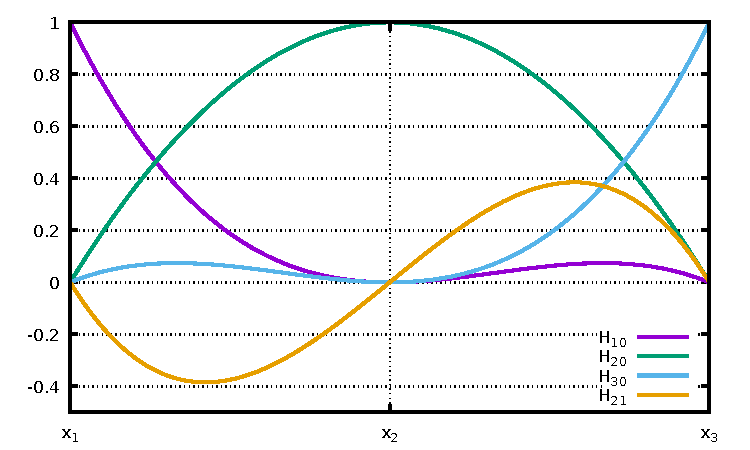
\includegraphics[width=.8\textwidth]{graph/interpolation/simpson}
    \caption{Basisfunktionen für die Simpsonregel. Beachte, dass $H_21$ in allen Quadraturpunkten verschwindet und auch das Integral null ist.}
    \label{fig:simpson}
  \end{figure}
  Die Funktion $H_{21}(x)$ ist das Produkt der Parabel
  $(x-x_1)(x-x_3)$, die symmetrisch zur Intervallmitte ist mit einer
  linearen Funktion mit Nullstelle in der Intervallmitte. Daher
  verschwindet ihr Integral und das zugehörige Integrationsgewicht ist
  null. Die Simpson-Regel lässt sich also schreiben als
  \begin{gather}
    Q_I = \frac h6f(x_1)+\frac{4h}6f(x_2) + \frac h6f(x_3) + 0 f'(x_2).
  \end{gather}
  Für die obige Interpolation gilt nach
  \slideref{Satz}{Hermite-restglied} die Fehlerdarstellung
  \begin{gather}
    f(x) - p(x) = \frac{f^{4}(\xi(x)}{4!} \pnewton_{x_1,x_2,x_2,x_3}(x).
  \end{gather}
  Integration ergibt
  \begin{align}
    \left|\int_I f\dx - Q_I(f)\right|
    &= \left|\int_I \bigl(f(x) - p(x)\bigr)\dx\right|\\
    &\le \max_{\xi\in I} \frac{f^{4}(\xi}{4!}
      \int_I \pnewton_{x_1,x_2,x_2,x_3}(x) \dx.
  \end{align}
  Schließlich berechnen wir
  \begin{gather}
    \int_I \pnewton_{x_1,x_2,x_2,x_3}(x) \dx
    = \int_I (x-x_1)(x-x_2)^2(x-x_3)
    = \frac1{120}
  \end{gather}
\end{proof}

\begin{remark}
  Ab Grad ??? haben die Newton-Cotes-Formeln negative Gewichte...
\end{remark}

\subsection{Gauß-Quadratur}

\begin{Lemma}{quadratur-exakt-max}
  Sei $Q_n$ eine Quadraturformel auf einem Intervall $I$ mit $n$
  Quadraturpunkten. Dann ist $Q_n$ maximal exakt vom Grad $2n-1$.
\end{Lemma}

\begin{proof}
  Siehe \cite[Satz 3.1]{Rannacher17}
\end{proof}

\begin{Definition}{Gauss-Legendre}
  Die $n$-Punkt-\define{Gauß-Legendre-Formel} auf dem Intervall
  $I=[-1,1]$ benutzt als Stützstellen $x_1,\dots,x_n$ die Nullstellen
  des Legendre-Polynoms $\plegendre(x)$ vom Grad $n$. Ihre
  Quadraturgewichte sind die Integrale der Lagrange-Polynome
  \begin{gather}
    \omega_i = \int_I \plagrange_{i;x_1,\dots,x_n}(x)\dx.
  \end{gather}
\end{Definition}

\begin{Satz}{gauss-legendre}
  Die $n$-Punkt-Gauß-Legendre-Formel ist wohldefiniert und exakt für
  beliebige Polynome vom Grad $2n-1$.
\end{Satz}

\begin{Satz}{gauss-legendre-eindeutig}
  Seien die Quadraturformeln $Q_k$ mit Quadraturpunkten
  $x_1^{(k)},\dots,x_k^{(k)}$ für $k=1,\dots,n$ auf dem Intervall
  $I=[-1,1]$ exakt für beliebige $p\in \P_{2k-1}$. Dann sind die
  Polynome
  \begin{gather}
    p_k(x) = \prod_{i=1}^k (x-x_i^{(k)}) \in \P_k
  \end{gather}
  und $p_0(x) = 1 \in \P_0$ paarweise orthogonal bezüglich des
  $L^2$-Skalarprodukts. Insbesondere sind sie damit Vielfache der
  Legendre-Polynome $\plegendre_k$ und die
  $n$-Punkt-Gauss-Legendre-Formel ist die einzige Formel mit $n$
  Punkten, deren Grad der Exaktheit $2n-1$ ist.
\end{Satz}

\begin{Lemma}{gauss-legendre-gewichte}
  Die Gewichte der Gauss-Legendre-Formeln sind positiv und genügen der
  Darstellung
  \begin{gather}
    \omega_i = \int_{-1}^1 \prod_{j\neq i}
    \left(\frac{x-x_j}{x_i-x_j}\right)^2\dx.
  \end{gather}
\end{Lemma}

\begin{Lemma}{gauss-legendre-fehler}
  Für die Gauss-Legendre-Formel mit $n$ Quadraturpunkten auf
  $I=[-1,1]$ gilt die Fehlerabschätzung
  \begin{gather}
    \left|\int_I f\dx - Q_n(f)\right|
    \le \max_{\xi\in I}\frac{f^{(2n)}(\xi)}{(2n)!}
    \int_{-1}^1 \prod_{i=1}^n(x-x_i)^2.
  \end{gather}
\end{Lemma}

\begin{remark}
  Alle Resultate dieses Abschnitts gelten für Skalarprodukte der Form
  \begin{gather}
    \scal(p,q) = \int_I \omega(x)p(x)q(x)\dx
  \end{gather}
  mit einer positiven Gewichtsfunktion $\omega(x)$, wenn man die
  Legendre-Polynome durch die entsprechenden orthogonalen Polynome
  ersetzt.
\end{remark}

\subsection{Richardson-Extrapolation und Romberg-Quadratur}

\begin{Definition}{richardson-extrapolation}
  Sei $T(h)$ eine numerische Methode zur Approximation des
  tatsächlichen Wertes $T(0)$ mit Diskretisierungsparameter $h$ und
  Fehlerabschätzung $\abs{T(h)-T(0)} = \bigo(h^p)$. Zur
  \define{Richardson-Extrapolation} wertet man diese Methode mit einer
  Schrittfolge $h_1, h_2,\ldots,h_n$ aus, so dass die Schrittweite
  (theoretisch) gegen null geht. Wertet man dann das
  Interpolationspolynom $p(h^p)$ an der Stelle $h=0$ aus, so bekommt
  man unter stärkeren Voraussetzungen die verbesserte Approximation
  \begin{gather}
    \abs{T(0)-p(0)} = \bigo(h^{np}).
  \end{gather}
\end{Definition}

\begin{remark}
  Tatsächlich genügt die einfache Fehlerabschätzung
  $\abs{T(h)-T(0)} = \bigo(h^p)$ nicht, um die behauptete
  Konvergenzordnung zu beweisen. Man benötigt eine asymptotische
  Fehlerentwicklung der Form
  \begin{gather}
    T(h)-T(0) = \tau_1 h^p + \tau_2 h^{2p} + \dots \tau_n h^{np}
    + \bigo(h^{(n+1)p}).
  \end{gather}
\end{remark}

\begin{Definition}{Romberg-quadratur}
  Die \define{Romberg-Quadratur} beruht auf einer summierten
  Quadraturformel $Q_h$ der Ordnung $h^p$, die für eine Folge von
  Schrittweiten $h_1,\dots, h_n$ angewandt wird. Aus diesen berechnet
  man mit dem \putindex{Neville}-Algorithmus Approximationen für
  $Q_0$.
\end{Definition}

\begin{Algorithmus*}{romberg}{Romberg-Quadratur}
  \lstinputlisting{code/romberg.py}
\end{Algorithmus*}

\subsection{Praktische Aspekte}

\begin{remark}
  Die Konvergenzabschätzungen der Form
  \begin{gather}
    \left|\int_I f\dx - Q_h(f)\right| \le c h^p \norm{f^{p+1}}_{\infty;I}
  \end{gather}
  verlieren ihren Nutzen für große $h$, wenn die Ableitungen von $f$
  wachsen. Schlimmstenfalls bekommt man dann aus der
  Interpolationseigenschaft noch immer
  \begin{gather}
    \left|\int_I f\dx - Q_h(f)\right| \le c \norm{f}_{\infty;I}.
  \end{gather}
  Es gibt aber keine Garantie, dass der Fehler bei feinerer
  Unterteilung schrumpft.
  
  Ist aber $f\in C^{p+1}(I)$, so gilt die obige Abschätzung für
  hinreichend kleine $h_1>h_2$ in der stärkeren Form
  \begin{gather}
    \left|\int_I f\dx - Q_{h_2}(f)\right|
    \approx \left(\frac{h_2}{h_1}\right)^p
    \left|\int_I f\dx - Q_{h_1}(f)\right|.
  \end{gather}
  Man spricht hier vom asymptotischen Bereich, für größere $h$ vom
  präasymptotischen Bereich.
\end{remark}

%%% Local Variables:
%%% mode: latex
%%% TeX-master: "main"
%%% End:


\chapter{Lösung linearer Gleichungssysteme}

\section{Vektor- und Matrixnormen}

\subsection{Vektor- und Matrixnormen, Eigenwerte}

\begin{Definition}{norm}
  Eine \define{Norm} $\norm{\cdot}$ auf dem Vektorraum $V$ ist eine Abbildung
  \begin{gather}
    \begin{split}
      \norm{\cdot}\colon V &\to \R\\
      x&\mapsto \norm{x}
    \end{split}
  \end{gather}
  mit den Eigenschaften
    \begin{xalignat}3
    &\text{Homogenität:}
    &\norm{\alpha x} &= \abs{\alpha}\norm{x}
    &\forall \alpha&\in\R,x\in V
    \\
    &\text{Dreiecksungleichung:}
    &\norm{x+y} &\le \norm{x}+\norm{y}
    &\forall x,y&\in V
    \\
    &\text{Definitheit:}
    &\norm{x} & \ge 0
    &\forall x&\in V
    \\
    &&\norm{x} &\neq 0
    &\forall x&\neq0
    \end{xalignat}
  Verzichtet man auf die zweite Definitheitsbedingung, so erhält man eine \define{Seminorm}.
\end{Definition}

\begin{Definition}{norm-aequivalenz}
  Sei $V$ ein reeller Vektorraum. Zwei Normen $\norm{\cdot}_X$ und
  $\norm{\cdot}_Y$ auf $V$ heißen äquivalent, wenn es Konstanten $c>0$
  und $C>0$ gibt, so dass
  \begin{gather}
    c \norm{v}_X \le \norm{v}_Y \le C \norm{v}_X
    \qquad\forall v\in V.
  \end{gather}
\end{Definition}

\begin{Definition}{rn-konvergenz}
  Eine Folge $\{x^{(k)}\}\subset \R^n$ für $k=1,2,\dots$ heißt
  \textbf{komponentenweise konvergent} gegen $x\in \R^n$, wenn gilt
  \begin{gather}
    \forall \epsilon>0\;
    \exists k_0\in \mathbb N\;
    \forall k\ge k_0, i=1,\dots,n
    : \abs{x^{(k)}_i - x_i} < \epsilon.
  \end{gather}
  Die Folge heißt konvergent unter der Norm $\norm{\cdot}$ wenn gilt
  \begin{gather}
    \forall \epsilon>0\;
    \exists k_0\in \mathbb N\;
    \forall k\ge k_0
    : \norm{x^{(k)} - x} < \epsilon.
  \end{gather}
\end{Definition}

\begin{Lemma}{norm-aequivalenz}
  Sei $\norm{\cdot}$ eine beliebige Norm auf $\R_n$. Dann ist die Abbildung
  \begin{gather}
    f\colon x \mapsto \norm{x}
  \end{gather}
  stetig bezüglich der komponentenweisen Konvergenz. Ferner ist die
  Norm $\norm{\cdot}$ äquivalent zur Maximumsnorm.
\end{Lemma}

\begin{proof}
  Für den ersten Teil ist zu zeigen, dass zu einer komponentenweise
  konvergenten Folge von Vektoren auch deren Norm konvergiert. Sei
  $\{x^{(k)}\}$ eine solche Folge und dazu $k_0$ so gewählt, dass
  \begin{gather}
    \max_{i=1,\dots,n}\left\lvert\left(x_i^{(k)}-x_i\right) \norm{e_i}\right\rvert
      < \frac\epsilon n
    \qquad \forall k\ge k_0.
  \end{gather}
  Hier ist $e_i$ der $i$-te Einheitsvektor. Dann folgt
  \begin{align}
    \norm{x^{(k)}-x}
    &= \left\lVert\sum_{i=1}^n \left(x_i^{(k)}-x_i\right) e_i\right\rVert
    \\
    &\le \sum_{i=1}^n \left\lVert\left(x_i^{(k)}-x_i\right) e_i\right\rVert
    \\
    & < n \frac\epsilon n = \epsilon.
  \end{align}
  Hiermit haben wir bereits bewiesen, dass komponentenweise Konvergenz
  auch Normkonvergenz impliziert.

  Die \glqq{}Einheitssphäre\grqq{}
   \begin{gather}
     S = \bigl\{ x\in \R^n \big| \norm{x}_\infty = 1 \bigr\}
   \end{gather}
   ist beschränkt und bezüglich der komponentenweisen Konvergenz
   abgeschlossen. Die Norm $\norm.$ nimmt dort als stetige Funktion
   ihr Minimum $c$ und ihr Maximum $C$ an. Insbesondere gilt aber
   wegen der Definitheit $c > 0$. Für einen beliebigen Vektor
   $x\in \R^n$ ist $x/\norm{x}_\infty \in S$, so dass gilt
   \begin{gather}
     c \norm{x}_\infty \le \norm{x} \le C \norm{x}_\infty.
   \end{gather}
\end{proof}

\begin{Satz}{norm-aequivalenz}
  Auf $\R^n$ sind zwei beliebige Normen $\norm._X$ und $\norm._Y$ äquivalent.
\end{Satz}

\begin{proof}
  Nach dem vorherigen Lemma sind beide Normen äquivalent zur Maximumsnorm. Es gibt also Konstanten $c_X, c_Y, C_X, C_y>0$ mit
  \begin{gather}
    \begin{aligned}
     c_X \norm{x}_\infty &\le &\norm{x}_X \;&\le C_X \norm{x}_\infty\\
     c_Y \norm{x}_\infty &\le &\norm{x}_Y \;&\le C_Y \norm{x}_\infty.
    \end{aligned}
  \end{gather}
  Daher gilt
  \begin{gather}
    \begin{split}
      \norm{x}_Y \le C_Y\norm{x}_\infty &\le \frac{C_Y}{c_X} \norm{x}_X\\
      \norm{x}_X \le C_X\norm{x}_\infty &\le \frac{C_X}{c_y} \norm{x}_Y
    \end{split}
  \end{gather}
\end{proof}


\begin{Definition}{matrix-norm}
  Auf dem Vektorraum der Matrizen $\R^{m\times n}$ ist durch
  \slideref{Definition}{norm} eine Norm definiert. Gilt zusätzlich
  \begin{gather}
    \norm{Ax} \le \norm{A}\norm{x}
    \qquad\forall A\in \R^{m\times n}, x\in \R^n,
  \end{gather}
  so heißt die Norm $\norm.$ der Matrix \define{verträglich} mit der
  Vektornorm $\norm.$. Wir sprechen von einer \define{Matrixnorm},
  wenn sie zusätzlich \define{submultiplikativ} ist, dass heißt,
  für alle Matrizen $A,B$ passender Dimensionen gilt
  \begin{gather}
    \norm{AB} \le \norm{A}\norm{B}.
  \end{gather}
  Ferner definieren wir die \define{Operatornorm} oder \define{natürliche Norm}
  \begin{gather}
    \norm{A} = \sup_{\substack{x\in\R^n\\x\neq0}} \frac{\norm{Ax}}{\norm{x}}
    = \sup_{\norm{x}=1}\norm{Ax}.
  \end{gather}
\end{Definition}

\begin{Lemma}{operator-norm}
  Die Operatornorm ist verträglich und submultiplikativ.
\end{Lemma}

\begin{Beispiel}{Zeilensummen}
  Die Operatornormen zu den Vektornormen $\norm._1$ und
  $\norm._\infty$ sind die \define{Spaltensummennorm} und die
  \define{Zeilensummennorm}
  \begin{align}
    \norm{A}_1 &= \max_{i=1,\dots,n} \sum_{j=1}^n \abs{a_{ji}}\\
    \norm{A}_\infty &= \max_{i=1,\dots,n} \sum_{j=1}^n \abs{a_{ij}}
  \end{align}
\end{Beispiel}

\begin{Definition}{eigenwert}
  Sei $A\in \R^{n\times n}$. Gilt für einen Vektor $0\neq x\in \R^n$
  \begin{gather}
    Ax = \lambda x,
  \end{gather}
  so nennen wir $\lambda$ \define{Eigenwert} von $A$ und $x$ einen
  zugehörigen \define{Eigenvektor}.
\end{Definition}

\begin{Lemma}{ew-norm}
  Für alle Eigenwerte $\lambda\in\C$ einer Matrix $A\in\R^{n\times n}$ gilt
  \begin{gather}
    \abs{\lambda} \le \norm{A}
  \end{gather}
  für jede zu einer beliebigen Vektornorm verträglichen Norm.
\end{Lemma}

\subsection{Konditionierung der Lösung}


%%% Local Variables:
%%% mode: latex
%%% TeX-master: "main"
%%% End:


\section{Die LR-Zerlegung}
\begin{Notation}{quadratische-matrizen}
  Da wir uns in diesem Abschnitt mit der Lösung quadraischer
  Gleichungssysteme beschäftigen, gelte für alle Matrizen, soweit
  nicht anders vermerkt, dass ihre Dimension $n\times n$ sei.
\end{Notation}

\subsection{Dreiecksmatrizen}

\begin{Definition}{dreiecksmatrix}
  Für eine \define{untere Dreiecksmatrix} $L \in \R^{n\times n}$ gilt
  \begin{gather}
    \ell_{ij} = 0,\qquad j>i.
  \end{gather}
  Für eine \define{obere Dreiecksmatrix} $R \in \R^{n\times n}$ gilt
  \begin{gather}
    r_{ij} = 0,\qquad j<i.
  \end{gather}
\end{Definition}

\begin{Satz}{dreieck-gruppe}
  Die Mengen der invertierbaren oberen und unteren Dreiecksmatrizen
  bilden jeweils eine multiplikative Gruppe. Die Determinante einer
  Dreiecksmatrix ist das Produkt ihrer Diagonalelemente.
\end{Satz}

\begin{proof}
  Hausaufgabe
\end{proof}

\begin{Korollar}{dreieck-inverse}
  Eine Dreiecksmatrix ist invertierbar genau dann, wenn alle ihre
  Diagonalelemente von null verschieden sind.
\end{Korollar}

\begin{Algorithmus}{vorwaerts-rueckwaerts}
  Die Lösung der linearen Gleichungssysteme
  \begin{gather}
    Lx = b \qquad Rx = b
  \end{gather}
  mit einer unteren Dreiecksmatrix $L$ und einer oberen Dreiecksmatrix
  $R$ lässt sich sukzessive durch Vorwärts- bzw.\ Rückwärtseinsetzen
  berechnen.
  \begin{minipage}[t]{.45\linewidth}
    \lstinputlisting[basicstyle=\footnotesize]{code/forsub.py}    
  \end{minipage}
  \begin{minipage}[t]{.45\linewidth}
    \lstinputlisting[basicstyle=\footnotesize]{code/backsub.py}    
  \end{minipage}
\end{Algorithmus}

\subsection{Konstruktion der LR-Zerlegung}

\begin{Definition}{frobenius-matrix}
  Eine Matrix der Gestalt
  \begin{gather}
    G_k=\begin{bmatrix}
      1 & & & & & \\
      &\ddots & & & & \\
      &   & 1& & &\\
      &   & g_{k+1,k}&1 & &\\
      &   & \vdots& &\ddots &\\
      &   & g_{nk}& & &1
    \end{bmatrix}
  \end{gather}
  mit von null verschiedenen Subdiagonaleinträgen nur in Spalte $k$
  heißt \define{Frobenius-Matrix}.
\end{Definition}

\begin{Lemma}{frobenius-matrix}
  Für Frobenius-Matrizen gilt
  \begin{gather}
    G_k^{-1} = 2\identity-G_k.
  \end{gather}
  Das Ergebnis des Produktes $G_kA$ einer Frobeniusmatrix mit einer
  beliebigen Matrix ergibt sich aus $A$ dadurch, dass auf die $j$-te
  Zeile das $g_{jk}$-fache der $k$-ten Zeile addiert wird.

  Sei $k_1<\dots<k_m$ eine aufsteigende Folge von Indizes. Dann ist
  \begin{gather}
    G_{k_1}\dots G_{k_m} = \sum_{i=1}^m G_i - (m-1) \identity.
  \end{gather}
  Insbesondere gilt
  \begin{gather}
    G_1\dots G_n =
    \begin{bmatrix}
      1\\
      g_{21} & 1 \\
      \vdots & \ddots & \ddots \\
      g_{n1}  & \dots & g_{n,n-1} & 1
    \end{bmatrix}
  \end{gather}
\end{Lemma}

\begin{Lemma}{elimination-1}
  Bei der Gauß-Elimination lässt sich die Elimination der
  Subdiagonalelemente der $k$-ten Spalte als Matrix-Produkt
  \begin{gather}
    A^{(k+1)} = L^{-1}_k A^{(k)},
    \qquad b^{(k+1)} = L^{-1}_k b^{(k)},
    \qquad k=1,\dots,n-1
  \end{gather}
  mit $A^{(1)}=A$, $b^{(1)}=b$ und den Frobenius-Matrizen
  \begin{gather}
    L_k =\begin{bmatrix}
      1 & & & & & \\
      &\ddots & & & & \\
      &   & 1& & &\\
      &   & \ell_{k+1,k}&1 & &\\
      &   & \vdots& &\ddots &\\
      &   & \ell_{nk}& & &1
    \end{bmatrix},
    \qquad
    \ell_{ik} = \frac{a_{ik}^{(k)}}{a_{kk}^{(k)}}
  \end{gather}
  schreiben.
\end{Lemma}

\begin{Lemma}{elimination-2}
  Nach $n-1$ Schritten der Gauß-Elminiation erhält man das transformierte lineare Gleichungssystem
  \begin{gather}
    R x = y,\qquad R = L^{-1}A, \qquad y=L^{-1}b,
    \qquad L = L_1^{-1}\cdot L_{n-1}^{-1} A
  \end{gather}
\end{Lemma}
\subsection{Fehleranalyse}


%%% Local Variables:
%%% mode: latex
%%% TeX-master: "main"
%%% End:


\section{Die QR-Zerlegung}
\subsection{Definition of the methods}

\begin{Algorithm*}{subspace-iteration}{Orthogonal subspace iteration}

  Let $\mata\in\Cnn$, $\matx_0 \in \C^{n\times m}$.\\
  For $k=0,\ldots$ until convergence repeat
  \begin{itemize}
  \item $\matz_k = \mata \matx_k$.
  \item $\matq_k\matr_k = \matz_k$ (QR factorization)
  \item $\matx_{k+1} = \matq_k$
  \end{itemize}
\end{Algorithm*}

\begin{Algorithm*}{qr-iteration}{QR iteration}
  
  Let $\mata_1 = \mata\in\Cnn$.\\
  For $k=1,\ldots$ until convergence repeat
  \begin{itemize}
  \item $\matq_k\matr_k = \mata_k$ (QR factorization)
  \item $\mata_{k+1} = \matr_k\matq_k$
  \end{itemize}
\end{Algorithm*}

\subsection{Analysis}
\begin{Theorem*}{schur-canonical}{Schur canonical form}
  For every matrix $\mata\in\Cnn$ there are a unitary matrix
  $\matq\in\Cnn$ and an upper triangular matrix $\matr\in\Cnn$ such
  that
  \begin{gather}
    \mata = \matq \matr \matq^*.
  \end{gather}
  The diagonal entries of $\matr$ are the eigenvalues of $A$. The
  column vectors of $\matq$ are called \define{Schur vectors}.
\end{Theorem*}

\begin{Lemma}{schur-canonical-1}
  For any $k\le n$ the span of the Schur vectors
  $\vq_1,\dots,\vq_k$ is invariant under the action of $\mata$.

  For $\matq_k = (\vq_1\dots\vq_k)$ and $R_k$ the upper left $k\times k$ block of $\matr$, there holds
  \begin{gather}
    \mata\matq_k = \matq_k \matr_k.
  \end{gather}
\end{Lemma}

\begin{Lemma}{schur-canonical-2}
  The Schur vectors depend on the order chosen for the eigenvalues,
  and in case of geometric multiplicity, the eigenvectors,
  respectively. They are determined up to factors $e^{i\phi}$
\end{Lemma}

\begin{Theorem}{convergence-subspace-iteration}
  Let $\mata\in\Cnn$ and
  \begin{gather}
    \abs{\lambda_1} >
    \abs{\lambda_2}>\dots>\abs{\lambda_m}>\abs{\lambda}
  \end{gather}
  for all
  remaining eigenvalues $\lambda\in\sigma(\mata)$. Let
  $\matq = (\vq_1\dots\vq_m)$ be the Schur vectors associated with the
  first $m$ eigenvalues and $\esp{1,\dots,j}$ be the space spanned by
  the first $j$ eigenvectors and $P_j$ the orthogonal projector
  onto this space. Let the set of start vectors of the orthogonal subspace iteration
  $\matx_0 = (\vx_1\dots\vx_m)$ be chosen that
  \begin{gather}
    \operatorname{span}\{P_1 \vx_1,\dots,P_j\vx_j\} = \esp{1,\dots,j},\qquad j=1,\dots,m.
  \end{gather}
  Then, the $j$-th column of $\matx_k$ converges to $\vq_j$ for $j=1,\dots,m$ up to a factor $e^{i\phi}$.
\end{Theorem}

\begin{Lemma}{qr-1}
  The matrices $\mata_k$ of the QR-iteration have the following properties:
  \begin{enumerate}
  \item $\mata_{k+1} = \matq_k^*\mata_k\matq_k = \matq_k^*\dots\matq_1^*A\matq_1\dots\matq_k$.
  \item $\mata^k=\matq_1\dots\matq_k\matr_k\dots\matr_1$.
  \item If $\mata$ is normal, so is $\mata_k$ for any $k$.
  \item If $\mata$ is symmetric, so is $\mata_k$ for any $k$.
  \end{enumerate}
\end{Lemma}

\begin{Theorem}{convergence-qr-iteration}
Removed
\end{Theorem}

\subsection{Implementation issues}
\begin{intro}
  In each step of the QR-iteration, a QR-decomposition of the matrix
  is needed, which requires $\bigo(n^3)$ operations. Thus, the
  complexity of the iteration is highly unfavorable. The following
  discussion will provide us with means to reduce the complexity of
  the QR-decomposition to $\bigo(n^2)$, in the symmetric case even to
  $\bigo(n)$.
\end{intro}

\begin{Definition}{hessenberg}
  A matrix is in \define{Hessenberg form} or is a \define{Hessenberg
    matrix}, if all its entries below the first subdiagonal are zero. Visually,
  \begin{gather}
    H = 
    \begin{pmatrix}
      *&*&*&*&*&*\\
      *&*&*&*&*&*\\
      0&*&*&*&*&*\\
      0&0&*&*&*&*\\
      0&0&0&*&*&*\\
      0&0&0&0&*&*
    \end{pmatrix}
  \end{gather}
  A symmetric or Hermitian Hessenberg matrix is \define{tridiagonal}.
\end{Definition}

\begin{Theorem}{Hessenberg-qr}
  The QR-decomposition of a Hessenberg matrix $\matH$ can be obtained
  by $n-1$ givens rotations. The matrix $\matr\matq$ is again in
  Hessenberg form. For a (complex) symmetric matrix $\matH$, the
  matrix $\matr\matq$ is even tridiagonal and (complex) symmetric.
\end{Theorem}

\begin{Corollary}{Hessenberg-qr}
  The complexity of each step of a QR-iteration for Hessenberg matrices is $\bigo(n^2)$. For tridiagonal (complex) symmetric matrices, it is $\bigo(n)$.
\end{Corollary}

\begin{Theorem}{Hessenberg-householder}
  Every matrix $\mata\in\Cnn$ is unitarily similar to a Hessenberg matrix $\matH$, that is,
  \begin{gather}
    \matH = \matq \mata \matq^*.
  \end{gather}
  The matrix $\matq$ can be obtained by $n-2$ \putindex{Householder
    reflections}.
\end{Theorem}

\begin{Algorithm*}{qr-method}{The QR-Method}
  Compute the spectrum of a matrix $\mata\in\Cnn$ by
  \begin{enumerate}
  \item Use $n-2$ Householder transformations to transform $\mata$ to
    Hessenberg form
    \begin{gather}
     \matH = \matq\mata\matq^*.
   \end{gather}
 \item QR-iteration: let $\matH_{0}=\matH$ and perform until convergence
   \begin{align}
     \Omega^{(k)}_{1,2}\times\dots\times\Omega^{(k)}_{n-1,n} \matr &= \matH_k\\
     \matH_{k+1} &= \matr \Omega^{(k)}_{1,2}\times\dots\times\Omega^{(k)}_{n-1,n}.
   \end{align}
 \item Store Householder vectors as well as $r$ and $c$ for each
   Givens rotation if the eigenvectors are desired in the end.
  \end{enumerate}
\end{Algorithm*}

\begin{Theorem}{hessenberg-qr-convergence}
    Let $\matH\in\Cnn$ be a Hessenberg matrix with eigenvalues such that
  \begin{gather}
    \abs{\lambda_1} >
    \abs{\lambda_2}>\dots>\abs{\lambda_n}.
  \end{gather}
  Then, the sequences of the QR-iteration admit the following estimates:
  \begin{align}
    \dist(\esp{1,\dots,j},\spann{\vq_1^{(k)},\dots,\vq_j^{(k)}}) &= \bigo \left(\abs*{\frac{\lambda_{j+1}}{\lambda_j}}^k\right),
    \\
    h_{j+1,j}^{(k)} &= \bigo \left(\abs*{\frac{\lambda_{j+1}}{\lambda_j}}^k\right)
                      .
  \end{align}
  Here, $h_{ij}^{(k)}$ are the entries of $\matH_k$.
\end{Theorem}

\begin{proof}
  See~\cite[Theorem 7.3-1]{GolubVanloan83}.
\end{proof}

\subsection{Shifts and deflation}

\begin{intro}
  The goal of this section is the development and justification of a
  method which accelerates convergence of the QR-iteration and
  reducing the effort at the same time. It is based on shifts, like
  for the simple or inverse power method. But, shifts are much more
  powerful here, since we compute not only ``converging subspace'',
  but also its complement.
\end{intro}

\begin{Theorem}{qr-reduction}
  Let the matrix $\matH^{(k)}\in\Cnn$ in the QR iteration be of the
  form
  \begin{gather}
    \matH^{(k)} =
    \begin{pmatrix}
      \matH_{11} & \mata_{12}\\0 & \matH_{22}
    \end{pmatrix}
  \end{gather}
  with Hessenberg matrices $\matH_{11}\in\C^{p\times p}$,
  $\matH_{22}\in \C^{n-p\times n-p}$ and an arbitrary matrix
  $\mata_{12}\in \C^{p\times n-p}$. Then, the matrix $\matq^{(k)}$
  decouples into two diagonal blocks and $\matH^{(k+1)}$ has the same
  form. Thus, the iteration decouples into two separate iterations.
\end{Theorem}

\begin{Definition}{hessenberg-unreduced}
  A Hessenberg matrix is called \define{unreduced} if all entries on
  the first subdiagonal are nonzero. It is called \define{reduced}
  otherwise.
\end{Definition}

\begin{Algorithm*}{shifted-qr-iteration}{QR iteration with shift}
  Let $\matH_1 = \matq_0^*\mata\matq_0\in\Cnn$.\\
  For $k=1,\ldots$ until convergence repeat
  \begin{itemize}
  \item $\matq_k\matr_k = \matH_k - \sigma\id$ (QR factorization)
  \item $\mata_{k+1} = \matr_k\matq_k + \sigma\id$
  \end{itemize}
\end{Algorithm*}




\subsection{Methods in real arithmetic}

\begin{Theorem*}{real-schur-form}{The real Schur form}
  For every matrix $\mata\in \Rnn$ there is an orthogonal matrix
  $\matq\in\Rnn$ and a matrix $\matr\in\Rnn$ such that
  \begin{gather}
    \mata = \matq\matr\matq^*,
    \qquad
    \matr =
    \begin{pmatrix}
      R_{11} &* & *&*\\
      &R_{22}&*&*\\
      &&\ddots&*\\
      &&& R_{jj}
    \end{pmatrix},
  \end{gather}
  where the diagonal blocks are either of dimension one containing the
  real eigenvalues or of dimension 2 for complex conjugate eigenvalue
  pairs.
\end{Theorem*}


%%% Local Variables:
%%% mode: latex
%%% TeX-master: "main"
%%% End:


\section{Lineare Ausgleichsrechnung}
\begin{intro}
  Die Methode der kleinsten Fehlerquadrate führt auf die Minimierungsaufgabe
  \begin{gather}
    \norm{Ax-b}_2 = \min.
  \end{gather}
\end{intro}

\begin{Satz}{normalengleichungen}
  Sei $A\in \R^{m\times n}$ mit $m\ge n$ und $b\in \R^m$. Dann ist
  $x\in\R^n$ genau dann eine Lösung des linearen Ausgleichsproblems
  \begin{gather}
    \norm{Ax-b}_2 = \min,
  \end{gather}
  wenn $x$ Lösung der \define{Normalengleichungen}
  \begin{gather}
    A^TA x = A^Tb
  \end{gather}
  ist. Insbesondere ist die Minimierungsaufgabe eindeutig lösbar, wenn
  $A$ vollen Rang hat.
\end{Satz}

\begin{remark}
  Wir können die Normalengleichungen lösen, indem wir die symmetrische Matrix $C = A^TA\in \R^{n\times n}$ berechnen und dann eines der Verfahren der vorigen Abschnitte auf diese Matrix anwenden.
  
  Das Lemma nach der nächsten Definition legt nahe, dass das keine gute Idee ist, da sich die Konditionszahl durch das Matrixprodukt quadriert und damit die Lösungsgenauigkeit leidet.  
\end{remark}

\begin{Definition}{condition-rectangular}
  Die Konditionszahl einer rechteckigen Matrix maximalen Rangs bezüglich der Operatornorm zur Vektornorm $\norm{\cdot}$ ist
  \begin{gather}
    \cond(A) = \frac{\sup_{\norm{x}=1}\norm{Ax}}{\inf_{\norm{x}=1}\norm{Ax}}.
    \end{gather}
  Die Definition ist konsistent zur Definition für invertierbare, quadratische Matrizen.
\end{Definition}

\begin{Lemma}{condition-squared}
  Für eine Matrix $A\in\R^{m\times n}$ maximalen Rangs mit $m\ge n$ gilt
  \begin{gather}
    \cond(A^TA) = \cond(A)^2.
  \end{gather}
\end{Lemma}

\begin{Lemma}{qr-rectangular}
  Zu jeder Matrix $A\in \R^{m\times n}$ maximalen Rangs mit $m\le n$
  gibt es eine QR-Zerlegung
  \begin{gather}
  A = QR
  \end{gather}
  mit einer oberen Dreiecksmatrix $R\in\R^{n\times n}$ und einer Matrix $Q\in\R^{m\times n}$, deren Spalten ein Orthonormalsystem bilden.
  Unter der Zusatzbedingung $r_{ii}>0$ ist
  diese Zerlegung eindeutig.
\end{Lemma}

\begin{Satz}
  Sei $QR=A$ eine QR-Zerlegung. Dann kann die Lösung der Normalengleichungenvberechnet werden durch die Lösung des Systems
  \begin{gather}
    Rx = Q^Tb.
  \end{gather}
\end{Satz}

\begin{proof}
  Einsetzen der QR-Zerlegung in die Normalengleichungen ergibt
  \begin{gather}
  R^TQ^TQR x = R^T R x = R^TQ^T b.
  \end{gather}
  Da $R^T$ invertierbar ist, können wir die Inverse von links anwenden und erhalten das Resultat.
\end{proof}

% \begin{Definition}{pseudo-inverse}
%   Die \define{Pseudoinverse} $A^\dagger\in \R^{n\times m}$ einer Matrix $A\in\R^{m\times n}$ ist definiert dadurch, dass $x=a^\dagger b$ die Lösung des Minimierungsproblems 
% \end{Definition}

%%% Local Variables:
%%% mode: latex
%%% TeX-master: "main"
%%% End:


\chapter{Iterationsverfahren}

\section{Grundlagen}
\begin{Definition}{kontraktion}
  Sei $M\subset\R^n$. Eine Abbildung $f\colon M\to M$ ist eine \define{Kontraktion} auf $M$, wenn es eine Konstante $\rho < 1$ gibt, so dass
  \begin{gather}
    \norm{f(x) - f(y)} \le \rho \norm{x-y} \qquad\forall x,y\in M.
  \end{gather}
\end{Definition}

\begin{Satz*}{bfs}{Banachscher Fixpunktsatz}
  Sei $f$ eine Kontraktion auf der abgeschlossenen Menge $M\subset\R^n$. Dann gibt es genau einen \define{Fixpunkt} $x\in M$, also
  \begin{gather}
    x = f(x).
  \end{gather}
\end{Satz*}

\begin{Satz}{optimize-solve}
  Sei $g\colon \R^n\to \R$. Dann gilt für eine Minimalstelle $x^*$ von $g$,
  also
  \begin{gather}
    x^* = \operatorname*{argmin}_{x\in\R^n} g(x),
  \end{gather}
  notwendig
  \begin{gather}
    \nabla g(x^*) = 0.
  \end{gather}
  Das Minimierungsproblem lässt sich also auf das Finden einer
  Nullstelle von $f\colon \R^n\to \R^n$ mit $f(x) = \nabla g(x)$
  reduzieren. Umgekehrt lässt sich die Aufgabe, eine Nullstelle einer
  Funktion $f\colon \R^n \to \R^n$ zu finden, durch die Minimierung
  des Funktionals $g(x) = \norm{f(x)}$ darstellen.
\end{Satz}

%%% Local Variables:
%%% mode: latex
%%% TeX-master: "main"
%%% End:


\section{Nichtlineare Gleichungssysteme}
\section{Das Newton-Verfahren}

\begin{Definition}{newton-verfahren}
  Das \define{Newton-Verfahren} ist ein Iterationsverfahren zum
  Auffinden einer Nullstelle einer Funktion $f\colon \R^n\to \R^n$. Zu
  einem Startwert $x^{(0)} \in \R^n$ berechnen sich die weiteren
  Iterierten durch
  \begin{gather}
    \label{eq:newton:1}
    x^{(k+1)} = x^{(k)} - \bigl(\nabla f(x^{(k)})\bigr)^{-1} f(x^{(k)}).
  \end{gather}
\end{Definition}

\begin{Algorithmus*}{newton}{Newton-Verfahren}
  \lstinputlisting[firstline=3,lastline=9]{code/newton.py} Die
  Parameter zu dieser Funktion sind der Startwert $x$, die Funktion
  $f(x)$, die Anwendung der inversen Ableitung
  \begin{gather}
    \operatorname{Dfinv}(x,r) = \bigl(\nabla f(x)\bigr)^{-1}r,
  \end{gather}
  sowie eine Toleranz als Abbruchkriterium.
\end{Algorithmus*}
\begin{Lemma}{newton-1}
  Sei $M\subset \R^n$ konvex. Sei $f\colon M\to \R^n$ stetig differenzierbar auf $M$ und die Ableitung genüge der Lipschitz-Abschätzung
  \begin{gather}
    \norm{\nabla f(x) - \nabla f(y)} \le \gamma \norm{x-y}
    \qquad \forall x,y\in M.
  \end{gather}
  mit einer Konstanten $\gamma$. Dann gilt für alle $x,y\in M$
  \begin{gather}
    \norm{f(x)-f(y) - \nabla f(y)(x-y)}
    \le \frac\gamma2 \norm{x-y}^2.
  \end{gather}
\end{Lemma}

\begin{proof}
  Wir folgen~\cite[Hilfssatz 5.3.1]{Stoer83}.
  Sei $\phi\colon[0,1] \to \R^n$ die Hilfsfunktion definiert durch
  \begin{gather}
    \phi(t) = f\bigl(y+t(x-y)\bigr),
  \end{gather}
  so dass
  \begin{gather}
    f(x)-f(y) - \nabla f(y)(x-y) = \phi(1) - \phi(0) - \phi'(0)
    = \int_0^1 (\phi'(t)-\phi'(0))\dt,
  \end{gather}
  denn nach der Kettenregel gilt
  \begin{gather}
    \phi'(t) = \nabla f\bigl(y+t(x-y)\bigr)(x-y).
  \end{gather}
  Den Integranden schätzen wir ab durch
  \begin{align}
    \norm{\phi'(t)-\phi'(0)}
    & = \norm{\Bigl(\nabla f\bigl(y-t(x-y)\bigr) - \nabla f(y)\Bigr)(x-y)}
    \\
    & \le \norm{\nabla f\bigl(y-t(x-y)\bigr) - \nabla f(y)}\norm{(x-y)}
    \\
    & \le \gamma\,t\norm{x-y}^2.
  \end{align}
  Einsetzen ins Integral ergibt
  \begin{gather}
    \norm{f(x)-f(y) - \nabla f(y)(x-y)}
    \le \frac\gamma2 \norm{x-y}^2.
  \end{gather}
\end{proof}

\begin{Satz}{newton-konvergenz}
  Sei $M\subset \R^n$ eine offene, konvexe Menge und
  $f\colon \overline{M} \to \R^n$ stetig differenzierbar in $M$ und
  stetig auf $\overline{M}$. Die \define{Jacobi-Matrix} $\nabla f(x)$
  sei auf ganz $M$ invertierbar und es gebe Konstanten $\beta$ und
  $\gamma$, so dass für $x,y\in M$ gilt
  \begin{gather}
    \label{eq:newton:2}
    \norm{\nabla f(x) - \nabla f(y)} \le \gamma \norm{x-y},
    \qquad \norm{\bigl(\nabla f(x)\bigr)^{-1}} \le \beta.
  \end{gather}
  Gibt es dann eine Konstante $\alpha$, so dass
  \begin{align}
    \label{eq:newton:3}
    \norm{\bigl(\nabla f(x^{(0)})\bigr)^{-1} f(x^{(0)})}
    &\le \alpha\\
    h := \frac{\alpha\beta\gamma}2 &<1\\
    \overline{B_r(x^{(0)})} &\subseteq M, \qquad\text{mit } r=\frac{\alpha}{1-h},
  \end{align}
  So ist die Folge $x^{(k)}$ des Newton-Verfahrens für alle
  $k=1,\dots$ wohldefiniert und liegt in $B_r(x^{(0)})$. Ferner
  konvergiert sie quadratisch gegen einen Wert
  $x^*\in\overline{B_r(x^{(0)})}$ und es gilt
  \begin{gather}
    \label{eq:newton:4}
    \norm{x^{(k)}-x^*} \le \alpha\frac{h^{2^k-1}}{1-h^{2^k}}.
  \end{gather}
\end{Satz}

\begin{proof}
  Wir folgen~\cite[Satz 5.3.2]{Stoer83}.
  Wir zeigen zunächst induktiv für alle $k=1,\dots$, dass das
  Folgenglied $x^{(k)}$ in $B_r(x^{(0)}) \subseteq M$ liegt. Damit
  existiert dann nach Voraussetzung
  $\bigl(\nabla f(x^{(k)})\bigr)^{-1}$ und $x^{(k+1)}$ ist
  wohldefiniert. Zur Verankerung bemerken wir, dass offensichtlich
  $x^{(0)}\in B_r(x^{(0)})$ und $x^{(1)}$ nach
  Voraussetzung~\eqref{eq:newton:3}. Nach der Verfahrensvorschrift
  können wir abschätzen:
  \begin{align}
    \norm{x^{(k+1)} - x^{(k)}}
    & = \norm{\bigl(\nabla f(x^{(k)})\bigr)^{-1} f(x^{(k)})}\\
    & \le \beta \norm{f(x^{(k)})}\\
    & = \beta \norm{f(x^{(k)}) - f(x^{(k-1)}) - \nabla f(x^{(k)})(x^{(k)}-x^{(k-1)})},
  \end{align}
  wobei wir die letzte Zeile aus der Multiplikation der
  Verfahrensvorschrift mit $\nabla f$ gewonnen haben. Hierauf wenden
  wir nun \slideref{Lemma}{newton-1} an und bekommen die quadratische
  Konvergenz, wenn der Abstand zweier Folgenglieder einmal klein genug
  ist:
  \begin{gather}
    \label{eq:newton:5}
    \norm{x^{(k+1)} - x^{(k)}}
    \le \frac{\beta\gamma}2 \norm{x^{(k)} - x^{(k-1)}}^2.
  \end{gather}
  Es bleibt zu zeigen, dass die Folge in $B_r(x^{(0)})$ bleibt. Dazu
  zeigen wir per Induktion, dass
  \begin{gather}
    \label{eq:newton:6}
    \norm{x^{(k+1)} - x^{(k)}} \le \alpha h^{2^k-1}.
  \end{gather}
  Für $k=0$ folgt $\norm{x^{(1)} - x^{(0)}} \le \alpha$ direkt
  aus~\eqref{eq:newton:3}. Für den Induktionsschritt benutzen wir
  unsere Konvergenzabschätzung~\eqref{eq:newton:5}:
  \begin{gather}
    \norm{x^{(k+1)} - x^{(k)}}
    \le \frac{\beta\gamma}2 \norm{x^{(k)} - x^{(k-1)}}^2
    \le \frac{\beta\gamma}2 (\alpha h^{2^{k-1}-1})^2
    = \frac{\alpha\beta\gamma}2 \alpha h^{2^k-2}
    = \alpha h^{2^k-1}.
  \end{gather}
  Nun können wir mit einer Teleskopsumme abschätzen
  \begin{align}
    \norm{x^{(k+1)} - x^{(0)}}
    &\le \sum_{j=0}^k \norm{x^{(j+1)} - x^{(j)}}\\
    & \le \alpha (1+h+h^3+h^7+\dots+h^{2^k-1})\\
    &<\frac\alpha{1-h} = r,
  \end{align}
  Aus~\eqref{eq:newton:6} folgt mit dieser Abschätzung, dass $x^{(k)}$
  Cauchy Folge ist und durch Grenzübergang die
  Abschätzung~\eqref{eq:newton:4}.
\end{proof}

\section{Abstiegsverfahren und Globalisierung}

\begin{intro}
  Die lokale Konvergenz ist beim Newtonverfahren ein großes Hindernis
  für die Anwendung. Wählt man den Startwert nicht im Einzugsbereich
  einer Nullstelle, so divergiert das Verfahren. Der Einzugsbereich,
  wie er sich aus dem Konvergenzsatz ergibt, ist dabei oft sehr klein
  und daher schwer zu finden.

  Ziel dieses Abschnitts ist daher, eine Modifikation des
  Newton-Verfahrens zu finden, die den Konvergenzbereich aufweitet,
  idealerweise sogar globale Konvergenz erzeugt. Solche Modifikationen
  findet man unter der Bezeichnung \define{Globalisierung}.
\end{intro}

\begin{Definition}{anstiegskegel}
  Sei $g\colon \R^n\to \R$ stetig differenzierbar. Dann definieren wir
  den Kegel positiven Anstiegs zum Parameter $\gamma$ als
  \begin{gather}
    S_\gamma(x) = \bigl\{ s\in\R^n \big|
    \norm{s} = 1 \;\wedge \;
    \nabla g(x)\cdot s \ge \gamma\norm{\nabla g(x)}
    \bigr\}.
  \end{gather}
  Die Richtung des steilsten Anstiegs im Punkt $x$ ist $\nabla g(x)$.
\end{Definition}

\begin{todo}
  Umgebung ``remark''.
\end{todo}
Da es sich um normierte Vektoren handelt, ist die Menge $S_\gamma(x)$
eigentlich kein Kegel, sondern eine Kugel in der Einheitssphäre mit
Zentrum im normierten Gradienten und Radius $\arccos \gamma$. Zusammen
mit den Skalierungsfaktoren, die unten eingeführt werden,
repräsentiert sie aber einen Kegel.


\begin{Lemma}{abstieg-reduktion}
  Sei $g\colon\R^n\to\R$ stetig differenzierbar und in einem Punkt
  $y\in\R^n$ gelte $\nabla g(y) \neq 0$. Dann gibt es eine Umgebung
  $U(y)$ und $\lambda>0$, so dass für alle $x\in U(y)$,
  $s\in S_\gamma(x)$ und $\mu\in [0,\lambda]$ gilt
  \begin{gather}
    g(x-\mu s) \le g(x) - \frac{\mu\gamma}4 \norm{\nabla g(y)}.
  \end{gather}
\end{Lemma}

\begin{proof}
  Wir definieren zunächst eine Umgebung um $y$ auf der sich die
  Gradienten nicht zu sehr unterscheiden:
  \begin{gather}
    \label{eq:newton:8}
    U_1(y) = \left\{
      x\in\R^n \middle| \;\norm{\nabla g(x)-\nabla g(y)} \le \frac\gamma4 \norm{\nabla g(y)}
      \right\}.
    \end{gather}
    Eine zweite Umgebung ist so gewählt, dass dort der Abstiegskegel
    in einem größeren Abstiegskegel im Punkt $y$ enthalten ist:
    \begin{gather}
      U_2(y) = \left\{
        x\in\R^n \middle| S_\gamma(x) \subseteq S_{\nicefrac\gamma2}(y)\right\}.
    \end{gather}

    Wähle nun $\lambda>0$, so dass
    \begin{gather}
      \overline{B_{2\lambda}(y)}\subseteq U_1(y) \cap U_2(y).
    \end{gather}
    und $U(y) = B_\lambda(y)$. Dann zeigen wir nun die Aussage für
    alle $x\in U(y)$, $s\in S_\gamma(x)$ und $\mu\in[0,\lambda]$. Nach
    dem Mittelwertsatz existiert $\theta\in(0,1)$ so dass
    \begin{gather}
      g(x)-g(x-\mu s) = \mu \nabla g(x-\theta\mu s)s.
    \end{gather}
    Wir formen weiter um:
    \begin{align}
      \nabla g(x-\theta\mu s)s
      &= \bigl(\nabla g(x-\theta\mu s) - \nabla g(y)\bigr)s + \nabla g(y)s\\
      &\ge -\frac{\gamma}4 \norm{\nabla g(y)}\norm{s} + \nabla g(y)s\\
      &\ge -\frac{\gamma}4 \norm{\nabla g(y)} + \frac\gamma2 \norm{\nabla g(y)}\\
      & \ge \frac\gamma4 \norm{\nabla g(y)}.
    \end{align}
\end{proof}

\begin{todo}
  Reihenfolge vertauschen  
\end{todo}

\begin{Definition}{abstiegsverfahren}
  Ein \define{Abstiegsverfahren} für eine stetig differenzierbare
  Funktion $g\colon \R^n\to\R$ ist eine Iterationsvorschrift aus den
  folgenden Schritten: gegeben $x^{(k)}$,
  \begin{enumerate}
  \item wähle $\gamma_k>\gamma>0$ und eine Abstiegsrichtung
    $s^{(k)} \in S_{\gamma_k}(x^{(k)})$.
  \item Wähle eine Schrittweite $\alpha_k>0$ und setze
    \begin{gather}
      x^{(k+1)} = x^{(k)} - \alpha_k s^{(k)},
    \end{gather}
    so dass die \define{Reduktionsbedingung}
    \begin{gather}
      \label{eq:newton:7}
      g\bigl(x^{(k+1)}\bigr)
      \le g\bigl(x^{(k)}\bigr) - \frac{\gamma_k\alpha_k}{4}\norm{\nabla g(x^{(k)})}
    \end{gather}
    gilt.
  \end{enumerate}
\end{Definition}

\begin{remark}
  Lemma \slideref{Lemma}{abstieg-reduktion} stellt sicher, dass es in
  jedem Schritt ein positives $\alpha_k$ gibt, das die Bedingung
  erfüllt.
\end{remark}

\begin{Beispiel*}{steepest-descent}{Verfahren des steilsten Abstiegs}
  Sei der Vektor $x^{(k)} \in\R^n$ gegeben, dann wähle
  $s^{(k)} = \nabla g(x^{(k)})$. Die Schrittweite $\alpha_k$ wird aus
  der eindimensionalen Minimierungsaufgabe (auch \define{line search}
  genannt)
  \begin{gather}
    \alpha_k = \operatorname*{argmin}_{\alpha>0}
    g\bigl(x^{(k)} - \alpha s^{(k)}\bigr)
  \end{gather}
  bestimmt. Danach setze
  \begin{gather}
    x^{(k+1)} = x^{(k)} - \alpha_k s^{(k)}.
  \end{gather}
\end{Beispiel*}

\begin{Satz}{abstieg-haeufung}
  Sei $g\colon \R^n\to \R$ und $x^{(0)} \in\R^n$ so gewählt, dass die Menge
  \begin{gather}
    K = \Bigl\{x\in\R^n \; \Big| \; g(x) \le g\bigl(x^{(0)}\bigr) \Bigr\}
  \end{gather}
  kompakt und $g$ stetig differenzierbar auf einer Umgebung von $K$
  ist. Dann besitzt die Folge $\{x^{(k)}\}$ des Abstiegsverfahrens
  mindestens einen Häufungspunkt in $K$. Gilt zusätzlich in der
  Umgebung eines Häufungspunkts $\gamma_k \ge \gamma>0$, so existiert
  $\alpha$, so dass $\alpha_k \ge \alpha>0$ gewählt werden kann. In
  diesem Fall ist der Häufungspunkt ein stationärer Punkt von $g$.
\end{Satz}

\begin{proof}
  Da die Folge monoton fällt, bleibt sie in $K$ und hat der
  Kompaktheit wegen mindestens einen Häufungspunkt $x^*$. Wir benennen
  nun ebenfalls mit $\{x^{(k)}\}$ ebenfalls eine Teilfolge, die gegen diesen
  Häufungspunkt konvergiert.

  Wir machen die Widerspruchsannahme, dass $x^*$ kein stationäre Punkt von $g$ ist, also
  \begin{gather}
    \nabla g(x^*) \neq 0.
  \end{gather}

  Wir bemerken, dass nach Voraussetzung $S_{\gamma_k}(x^*) \subseteq S_\gamma(x^*)$ gilt.
  Nun gibt es nach \slideref{Lemma}{abstieg-reduktion} eine Umgebung
  $U(x^*)$ und eine Zahl $\lambda>0$, so dass für alle $\mu\in[0,\lambda]$ gilt:
  \begin{gather}
    g(x-\mu s) \le g(x) - \mu \frac\gamma4\norm{\nabla g(x^*)}.
  \end{gather}
  Daraus folgt, dass zu jedem $\alpha_k \le \lambda$ die
  Reduktionsbedingung~\eqref{eq:newton:7} erfüllt ist und
  dementsprechend die Bedingung $\alpha_k\ge\alpha$ für
  $\alpha\le\lambda$ erfüllt werden kann.

  Sei nun $k_0$ gewählt, so dass $x^{(k)}\in U(x^*)$ für alle
  $k\ge k_0$. Dann gilt nach der Konstruktion von $U(x^*)$
  in~\eqref{eq:newton:8}, dass
  \begin{gather}
    \norm{\nabla g(x^{(k)})} \ge \norm{\nabla g(x^{*})} - \norm{\nabla g(x^{(k)}) - \nabla g(x^{*})}
    \ge \left(1-\frac\gamma4\right)  \norm{\nabla g(x^{*})}.
  \end{gather}
  Es gilt also
  \begin{gather}
    g(x^{k+1}) \le g(x^{k}) - \frac34 \alpha \norm{\nabla g(x^{*})}.
  \end{gather}
  Daraus folgt im Widerspruch zur Stetigkeit die Konvergenz
  $g(x^{(k)}) \to -\infty$, Es muss also $\nabla g(x^{*})=0$ gelten,
  $x^*$ ist also ein stationärer Punkt von $g$.
\end{proof}

\begin{remark}
  Der vorherige besteht aus zwei Teilen. Die Existenz eines
  Häufungspunktes wird unter einer der allgemeinen Bedingung
  getroffen, dass die Menge $K$ kompakt ist, also eine Abstiegsfolge
  nicht ins unendliche konvergieren kann. Diese Bedingung ist oft
  recht leicht nachzuprüfen. Insbesondere steht die Existenz mehrerer
  Häufungspunkte nicht im Widerspruch zu den Annahmen, so dass das
  Verfahren auch dann wenigstens einen davon findet.

  Die weiteren Bedingungen, die sicherstellen, dass es sich bei einem
  Häufungspunkt um einen stationären Punkt handelt, sind lokal in
  einer Umgebung eines solchen gestellt. An diesem Punkt sind die
  Folgen $\gamma_k$ und $\alpha_k$ nur sehr abstrakt fixiert. Wir
  zeigen nun, dass die Folge der $\alpha_k$ im Verfahren des steilsten
  Abstiegs die Bedingung erfüllt. Als zweite Anwendung von allgemeinen
  Abstiegsverfahren stellen wir dann das Newton-Verfahren mit
  Schrittweitensteuerung vor.
\end{remark}

\begin{Korollar}{abstieg-haeufung}
  Beim Verfahren des steilsten Abstiegs sind die Folgen $\gamma_k$ und
  $\alpha_k$ so gewählt, das \slideref{Satz}{abstieg-haeufung} gilt.
\end{Korollar}

\begin{proof}
  Da die Abstiegsrichtungen immer gleich dem (negativen) Gradienten
  sind, gilt $\gamma_k \equiv 1$. Für die Folge $\alpha_k$ zeigen wir
  nich die Beschränktheit durch $\alpha$. Stattdessen bemerken wir mit
  $\lambda$ aus \slideref{Lemma}{abstieg-reduktion}:
  \begin{align}
    g(x^{(k+1)})
    &= \min_{\alpha>0} g\left(x^{(k+1)}-\alpha s^{(k)}\right)\\
    &\le g(x^{(k)}-\lambda s^{(k)})\\
    &\le g(x^{(k)}) - \frac{\lambda}4 \norm{\nabla g(x^*)}.
  \end{align}
  Auch hier schließen wir, dass die Folge divergiert wenn die Punkte konvergieren.
\end{proof}

\begin{Lemma}{newton-abstieg}
  Sei $f\colon \R^n\to \R^n$ stetig differenzierbar und
  $g(x) = \norm{f(x)}_2^2$.  Dann sind die Suchrichtungen des Newton-Verfahrens
  \begin{gather}
    s^{(k)} = \frac{d^{(k)}}{\norm{d^{(k)}}_2},
    \qquad d^{(k)} = \bigl(\nabla f(x^{(k)})\bigr)^{-1}f(x^{(k)})
  \end{gather}
  Abstiegsrichtungen für $g(x)$ und es gilt
  \begin{gather}
    s^{(k)} \in S_\gamma\bigl(x^{(k)}\bigr),
    \qquad
    \gamma = \frac{1}{\cond_2(\nabla f(x^{(k)}))}
  \end{gather}
\end{Lemma}

\begin{proof}
  Es gilt (Nachrechnen!)
  \begin{gather}
    \nabla g(x) = 2 f(x)^T\nabla f(x).
  \end{gather}
  Daher ist
  \begin{align}
    \frac{\nabla g(x) s}{\norm{\nabla g(x)}_2}
    &= \frac{f(x)^T \nabla f(x) \bigl(\nabla f(c)\bigr)^{-1} f(x)}
      {\norm{f(x)^T\nabla f(x)}_2\norm{\bigl(\nabla f(c)\bigr)^{-1} f(x)}}_2\\
    &\ge \frac{\norm{f(x)}^2_2}{\norm{f(x)}_2\norm{\nabla f(x)}_2\norm{\bigl(\nabla f(c)\bigr)^{-1}}_2\norm{f(x)}_2}\\
    &= \frac1{\cond_2(\nabla f)}.
  \end{align}
\end{proof}

\begin{Korollar}{newton-abstieg}
  Das modifizierte Newton-Verfahren
  \begin{gather}
    x^{(k+1)} = x^{(k)} - \alpha_k \bigl(\nabla f(x^{(k)})\bigr)^{-1} f(x^{(k)})
  \end{gather}
  ist ein Abstiegsverfahren, wenn $\alpha_k$ so gewählt ist, dass die
  Reduktionsbedingung gilt.
\end{Korollar}

\begin{remark}
  Man kann nun zum Beispiel auch das Newton-Verfahren mit line search
  ausführen, um globale Konvergenzeigenschaften zu erzielen. Es gilt
  dann zunächst die Existenz von Häufungspunkten. In der Nähe eines
  solchen gilt aber natürlich, dass line search nicht schlechter
  konvergiert, als das normale Newton-Verfahren, woraus dann dort
  wieder die quadratische Konvergenz gefolgert werden kann.

  Wir betrachten stattdessen die folgende, einfachere Variante, die
  mit minimaler Modifikation ein global konvergierendes Verfahren
  ergibt.
\end{remark}

\begin{Definition}{newton-stepsize}
  Das Newton-Verfahren mit \define{Schrittweitensteuerung} berechnet iterativ
  $x^{(k+1)}\in \R^n$ aus $x^{(k)}\in \R^n$ in folgenden Schritten
  \begin{enumerate}
  \item Berechne $d^{(k)} = \bigl(\nabla f(x^{(k)})\bigr)^{-1}f(x^{(k)})$
  \item Berechne die kleinste ganze Zahl $j$, so dass
    \begin{multline}
      \norm*{f(x^{(k)}-2^{-j} d^{(k)})}_2^2
      \le \norm*{f(x^{(k)})}_2^2
      \\- 2^{-j} \frac{1}{4\cond_2(\nabla f(x^{(k)}))}
      \norm*{f^T\bigl(x^{(k)}\bigr)\nabla f\bigl(x^{(k)}\bigr)}_2
    \end{multline}
    \item Setze $x^{(k+1)}=x^{(k)}-2^{-j} d^{(k)}$
  \end{enumerate}
\end{Definition}

\begin{remark}
  Der Algorithmus benötigt viele zusätzliche Berechnungen, wie die von
  $\gamma_k$ oder $\nabla g$. Für die praktische Anwendung lässt er
  sich vereinfachen. Dazu beobachten wir zunächst, dass
  Bedingung~\eqref{eq:newton:7} dazu dient, eine hinreichende
  Kontraktion in der Nähe eines Häufungspunkts sicherzustellen. Die
  Existenz eines solchen kann bereits aus
  \begin{gather}
    g\bigl(x^{k+1}\bigr) < g\bigl(x^{k}\bigr)
  \end{gather}
  gefolgert werden. Umgekehrt wird, wenn die Funktion $f$ die
  Bedingungen des Konvergenzsatzes \slideref{Satz}{newton-konvergenz}
  erfüllt, in der Nähe eines Fixpunktes ohnehin $j=0$ gelten. Wir
  ersetzen daher die komplizierte Bedingung durch die wesentlich
  einfachere: sei $j$ die kleinste nichtnegative ganze Zahl, so dass
  \begin{gather}
    \norm*{f\bigl(x^{k} - 2^{-j} d^{(k)}\bigr)}_2^2 < \norm*{f\bigl(x^{k}\bigr)}_2^2.
  \end{gather}
  Es gibt in der Literatur weitere Heuristiken zur Wahl der
  Schrittweite im Newton-Verfahren, die man unter dem Stichwort \glqq
  Globalisierung\grqq{} findet. Hier wollen wir uns mit dieser
  besonders einfachen und gleichzeitig effektiven Variante begnügen.
\end{remark}

\begin{Algorithmus*}{newton-stepsize}{Newton-Verfahren mit Schrittweitensteuerung}
    \lstinputlisting[firstline=3,lastline=18]{code/newton-stepsize.py}
\end{Algorithmus*}

\begin{remark}
  Dieser Abschnitt gibt Hinweise darauf, wie das Newton-Verfahren
  modifiziert werden kann und trotzdem Konvergenz erhalten wird. Neben
  der Schrittweitensteuerung kommen hier insbesondere approximative
  Berechnungen der Ableitung in Frage. Diese werden dann oft als
  \define{Quasi-Newton-Verfahren} bezeichnet, konvergieren in der
  Regel nur von erster Ordnung, sind aber of viel effizienter als das
  Newton-Verfahren selbst.
\end{remark}

%%% Local Variables:
%%% mode: latex
%%% TeX-master: "main"
%%% End:


\section{Dünnbesetzte lineare Gleichungssysteme}


\bibliographystyle{apalike}
\bibliography{all}
\printindex

%%% Local Variables:
%%% mode: latex
%%% TeX-master: "main"
%%% End:
